\documentclass[11pt]{article}
\usepackage[textwidth=18.0cm, textheight=23.0cm, top=2.0cm]{geometry}
\usepackage{pst-all}
\usepackage{amssymb}
\usepackage{tikz}
\usepackage{underscore}\begin{document}
\pagestyle{empty}


ClassName: \underline{\textbf{Class_08.2bp-38}}
\par
BinSize: \underline{\textbf{100 × 100}}
\par
ReduceSize: \underline{\textbf{100 × 100}}
\par
TypeNum: \underline{\textbf{80}}
\par
Num: \underline{\textbf{80}}
\par
OutS: \underline{\textbf{210000}}
\par
InS: \underline{\textbf{188362}}
\par
Rate: \underline{\textbf{0.897}}
\par
UB: \underline{\textbf{21}}
\par
LB0: \underline{\textbf{21}}
\par
LB: \underline{\textbf{21}}
\par
LBWithCut: \underline{\textbf{21}}
\par
NodeCut: \underline{\textbf{0}}
\par
ExtendedNodeCnt: \underline{\textbf{1}}
\par
GenNodeCnt: \underline{\textbf{1}}
\par
PrimalNode: \underline{\textbf{0}}
\par
ColumnCount: \underline{\textbf{21}}
\par
TotalCutCount: \underline{\textbf{0}}
\par
RootCutCount: \underline{\textbf{0}}
\par
LPSolverCnt: \underline{\textbf{1}}
\par
PricingSolverCnt: \underline{\textbf{0}}
\par
BranchAndBoundNum: \underline{\textbf{1}}
\par
isOpt: \underline{\textbf{true}}
\par
TimeOnInitSolution: \underline{\textbf{0.620 s}}
\par
TimeOnPrimal: \underline{\textbf{0.000 s}}
\par
TimeOnPricing: \underline{\textbf{0.000 s}}
\par
TimeOnRmp: \underline{\textbf{0.062 s}}
\par
TotalTime: \underline{\textbf{0.745 s}}
\par
\newpage


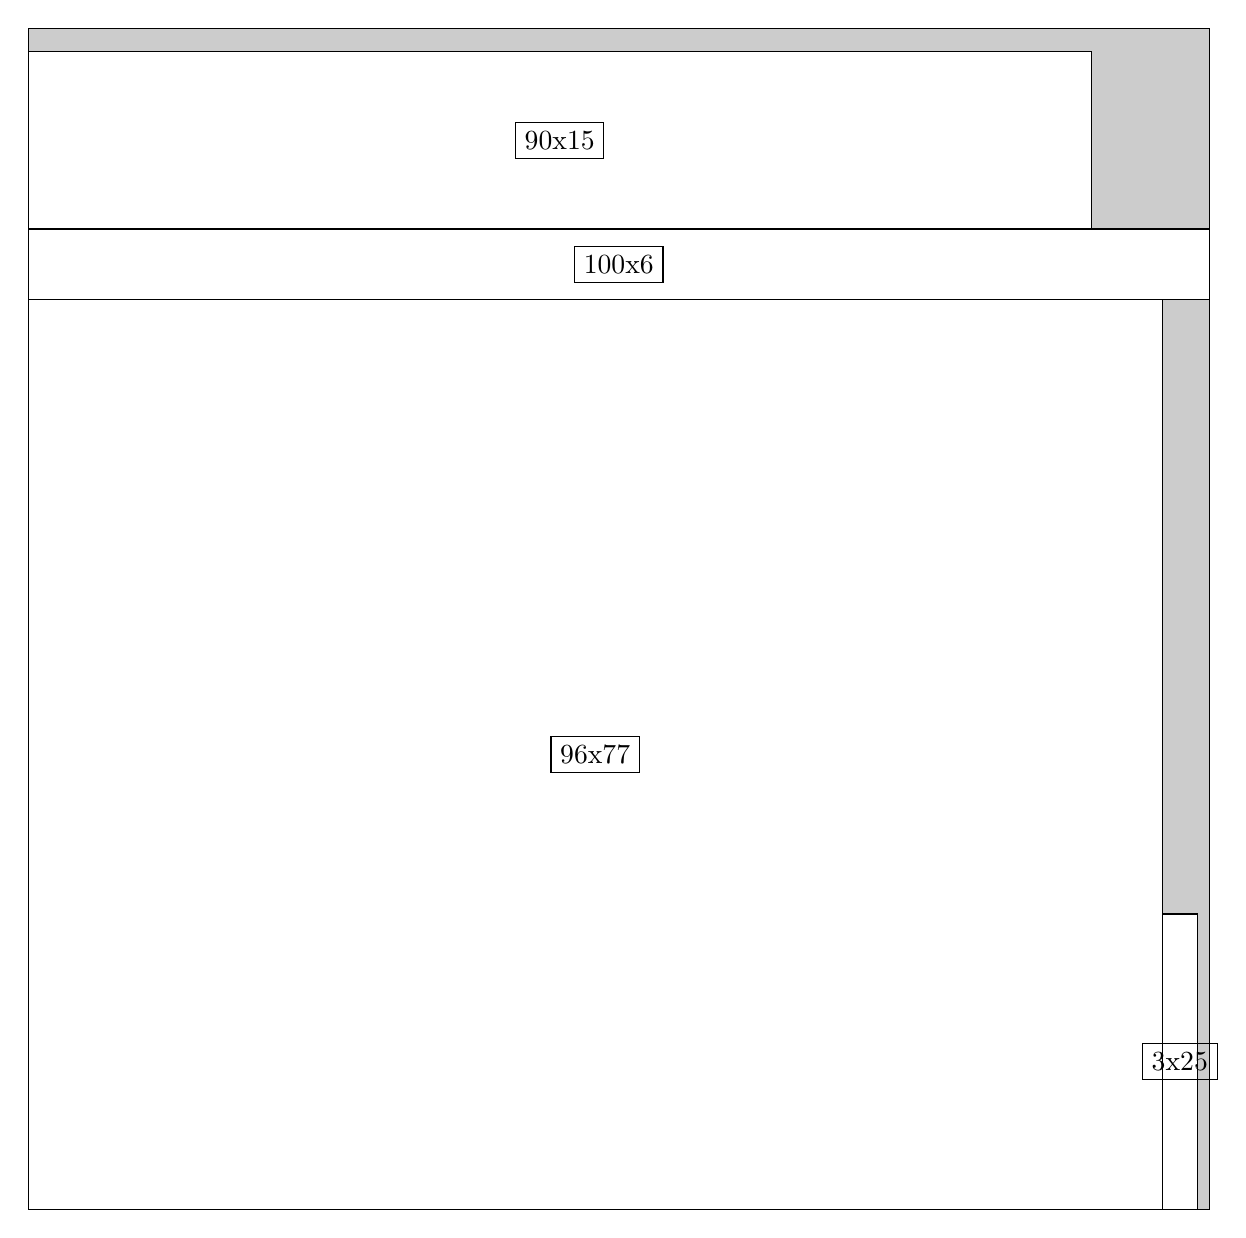
\begin{tikzpicture}[shorten >=1pt,scale=1.0,every node/.style={scale=1.0},->]
\tikzstyle{vertex}=[circle,fill=black!25,minimum size=14pt,inner sep=0pt]
\filldraw[fill=gray!40!white, draw=black] (0,0) rectangle (15.0,15.0);
\foreach \name/\x/\y/\w/\h in {96x77/0.0/0.0/14.399999999999999/11.549999999999999,90x15/0.0/12.45/13.5/2.25,100x6/0.0/11.549999999999999/15.0/0.8999999999999999,3x25/14.399999999999999/0.0/0.44999999999999996/3.75}
\filldraw[fill=white!40!white, draw=black] (\x,\y) rectangle node[draw] (\name) {\name} ++(\w,\h);
\end{tikzpicture}


w =96 , h =77 , x =0 , y =0 , v =7392
\par
w =90 , h =15 , x =0 , y =83 , v =1350
\par
w =100 , h =6 , x =0 , y =77 , v =600
\par
w =3 , h =25 , x =96 , y =0 , v =75
\par
\newpage


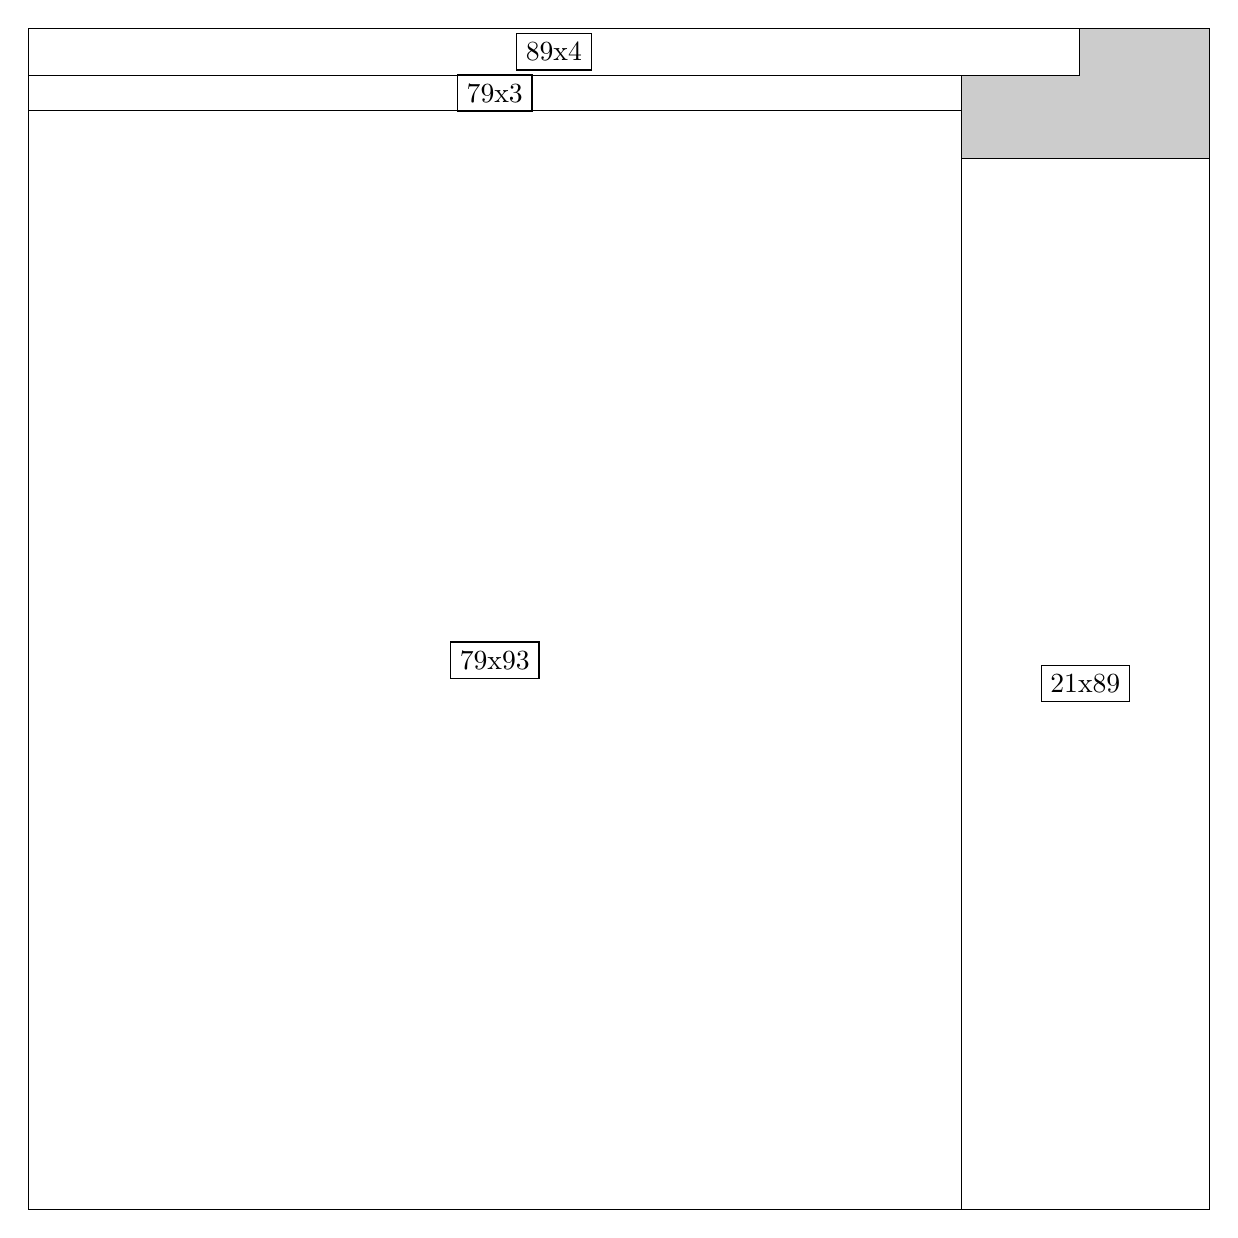
\begin{tikzpicture}[shorten >=1pt,scale=1.0,every node/.style={scale=1.0},->]
\tikzstyle{vertex}=[circle,fill=black!25,minimum size=14pt,inner sep=0pt]
\filldraw[fill=gray!40!white, draw=black] (0,0) rectangle (15.0,15.0);
\foreach \name/\x/\y/\w/\h in {79x93/0.0/0.0/11.85/13.95,21x89/11.85/0.0/3.15/13.35,89x4/0.0/14.399999999999999/13.35/0.6,79x3/0.0/13.95/11.85/0.44999999999999996}
\filldraw[fill=white!40!white, draw=black] (\x,\y) rectangle node[draw] (\name) {\name} ++(\w,\h);
\end{tikzpicture}


w =79 , h =93 , x =0 , y =0 , v =7347
\par
w =21 , h =89 , x =79 , y =0 , v =1869
\par
w =89 , h =4 , x =0 , y =96 , v =356
\par
w =79 , h =3 , x =0 , y =93 , v =237
\par
\newpage


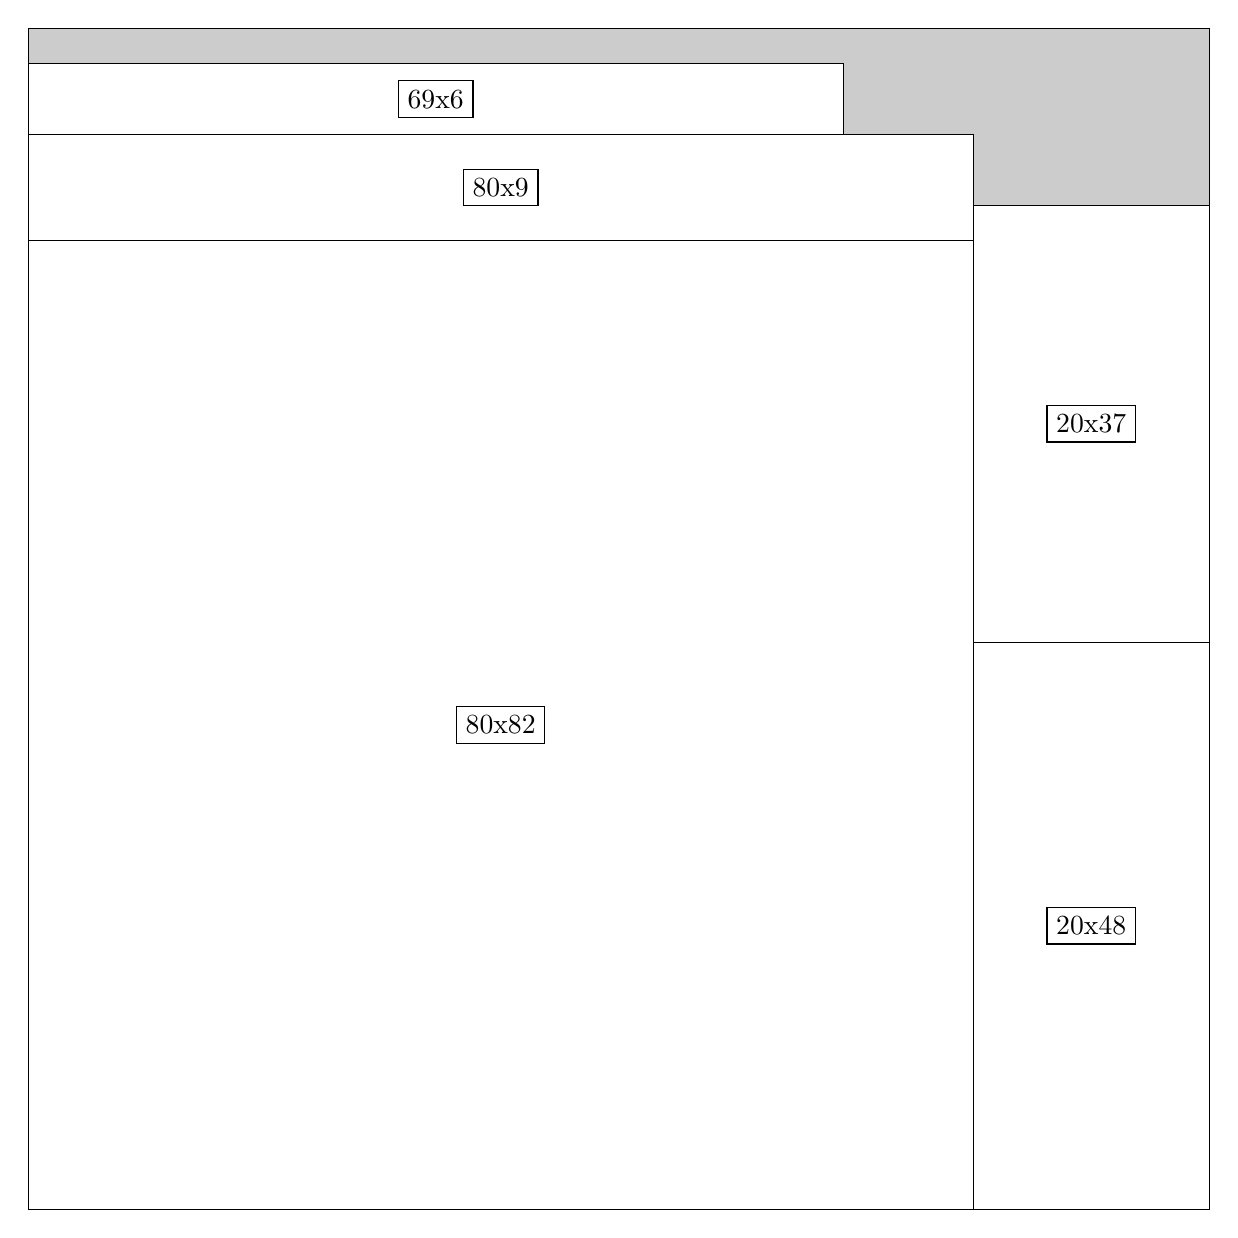
\begin{tikzpicture}[shorten >=1pt,scale=1.0,every node/.style={scale=1.0},->]
\tikzstyle{vertex}=[circle,fill=black!25,minimum size=14pt,inner sep=0pt]
\filldraw[fill=gray!40!white, draw=black] (0,0) rectangle (15.0,15.0);
\foreach \name/\x/\y/\w/\h in {80x82/0.0/0.0/12.0/12.299999999999999,20x48/12.0/0.0/3.0/7.199999999999999,20x37/12.0/7.199999999999999/3.0/5.55,80x9/0.0/12.299999999999999/12.0/1.3499999999999999,69x6/0.0/13.65/10.35/0.8999999999999999}
\filldraw[fill=white!40!white, draw=black] (\x,\y) rectangle node[draw] (\name) {\name} ++(\w,\h);
\end{tikzpicture}


w =80 , h =82 , x =0 , y =0 , v =6560
\par
w =20 , h =48 , x =80 , y =0 , v =960
\par
w =20 , h =37 , x =80 , y =48 , v =740
\par
w =80 , h =9 , x =0 , y =82 , v =720
\par
w =69 , h =6 , x =0 , y =91 , v =414
\par
\newpage


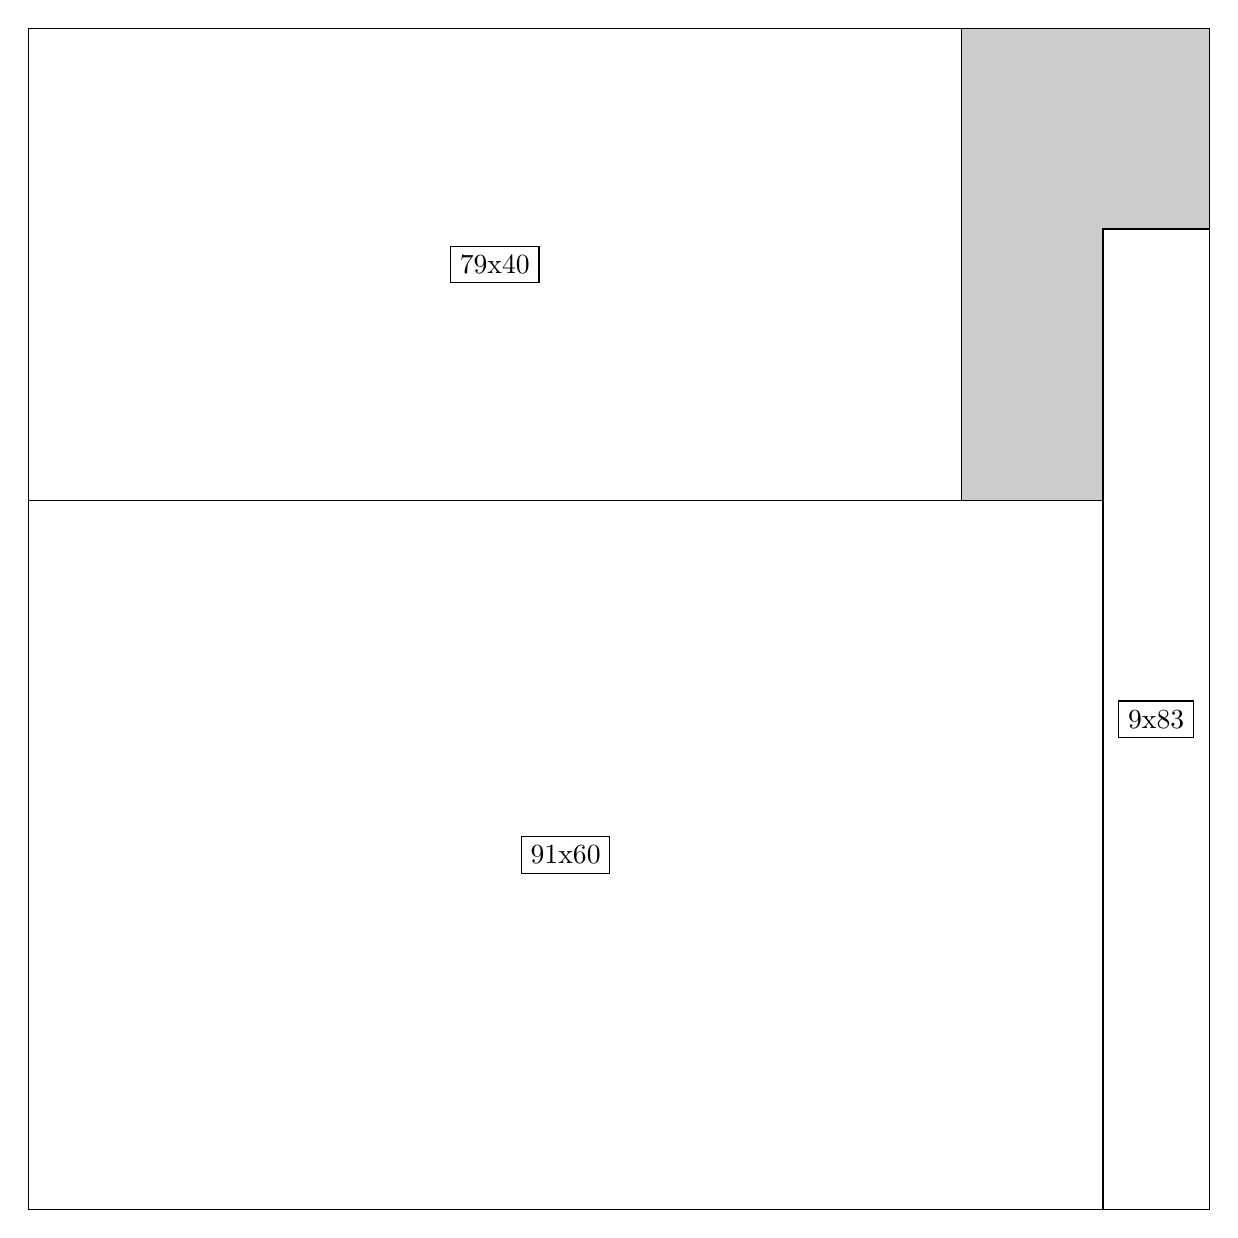
\begin{tikzpicture}[shorten >=1pt,scale=1.0,every node/.style={scale=1.0},->]
\tikzstyle{vertex}=[circle,fill=black!25,minimum size=14pt,inner sep=0pt]
\filldraw[fill=gray!40!white, draw=black] (0,0) rectangle (15.0,15.0);
\foreach \name/\x/\y/\w/\h in {91x60/0.0/0.0/13.65/9.0,79x40/0.0/9.0/11.85/6.0,9x83/13.65/0.0/1.3499999999999999/12.45}
\filldraw[fill=white!40!white, draw=black] (\x,\y) rectangle node[draw] (\name) {\name} ++(\w,\h);
\end{tikzpicture}


w =91 , h =60 , x =0 , y =0 , v =5460
\par
w =79 , h =40 , x =0 , y =60 , v =3160
\par
w =9 , h =83 , x =91 , y =0 , v =747
\par
\newpage


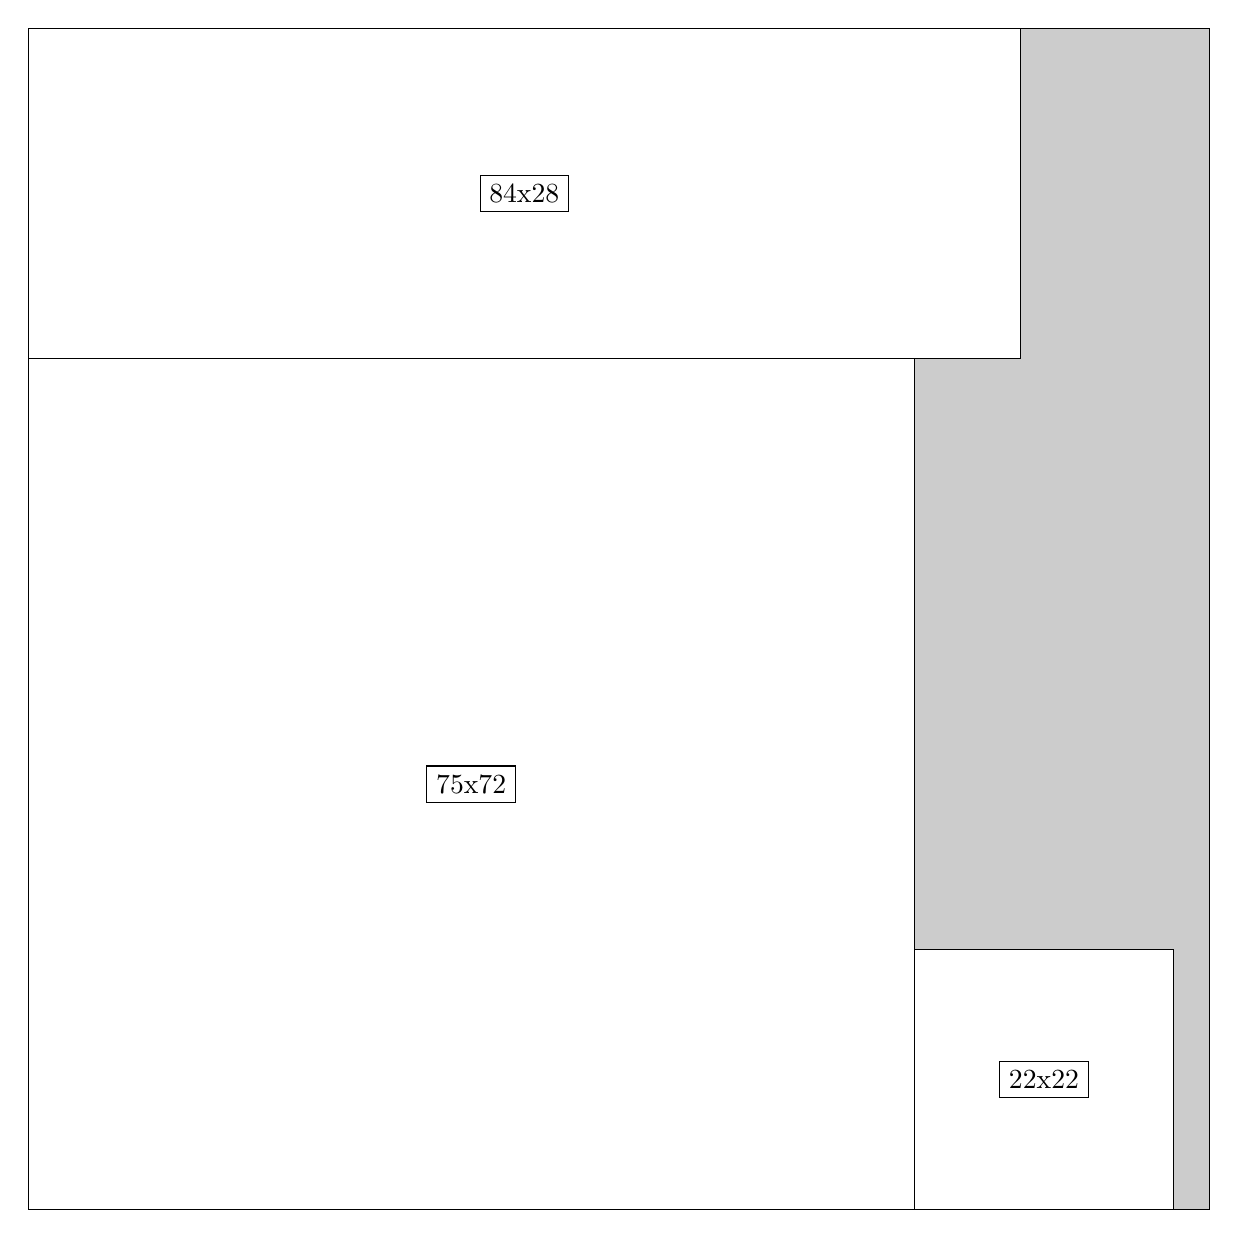
\begin{tikzpicture}[shorten >=1pt,scale=1.0,every node/.style={scale=1.0},->]
\tikzstyle{vertex}=[circle,fill=black!25,minimum size=14pt,inner sep=0pt]
\filldraw[fill=gray!40!white, draw=black] (0,0) rectangle (15.0,15.0);
\foreach \name/\x/\y/\w/\h in {75x72/0.0/0.0/11.25/10.799999999999999,84x28/0.0/10.799999999999999/12.6/4.2,22x22/11.25/0.0/3.3/3.3}
\filldraw[fill=white!40!white, draw=black] (\x,\y) rectangle node[draw] (\name) {\name} ++(\w,\h);
\end{tikzpicture}


w =75 , h =72 , x =0 , y =0 , v =5400
\par
w =84 , h =28 , x =0 , y =72 , v =2352
\par
w =22 , h =22 , x =75 , y =0 , v =484
\par
\newpage


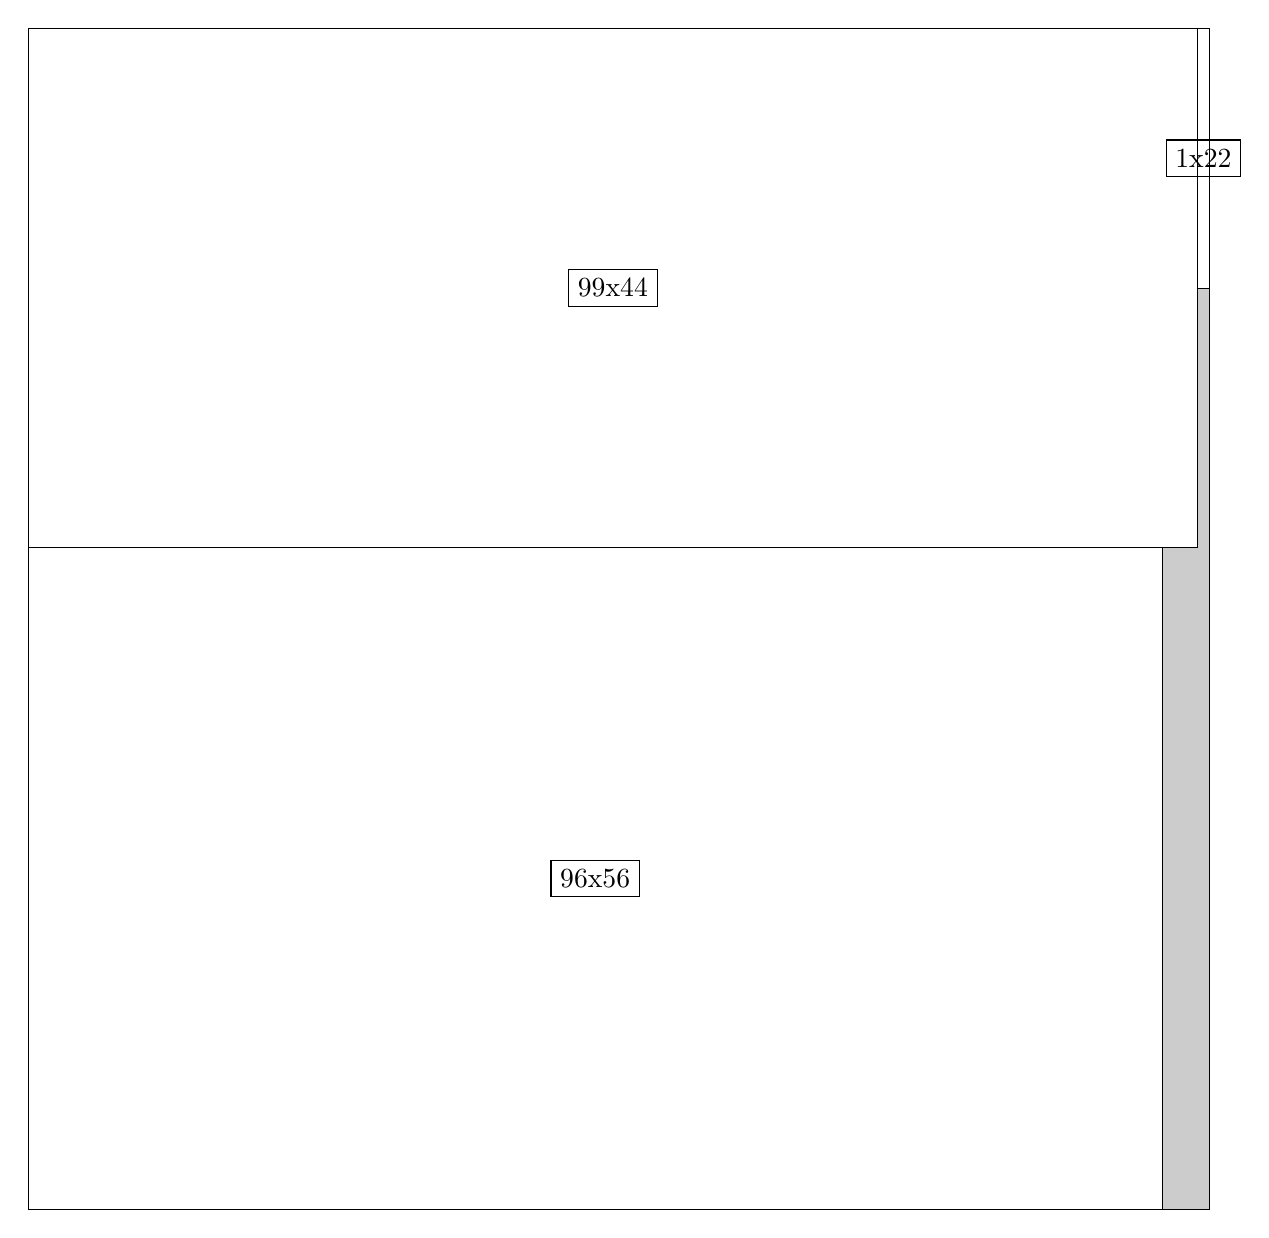
\begin{tikzpicture}[shorten >=1pt,scale=1.0,every node/.style={scale=1.0},->]
\tikzstyle{vertex}=[circle,fill=black!25,minimum size=14pt,inner sep=0pt]
\filldraw[fill=gray!40!white, draw=black] (0,0) rectangle (15.0,15.0);
\foreach \name/\x/\y/\w/\h in {96x56/0.0/0.0/14.399999999999999/8.4,99x44/0.0/8.4/14.85/6.6,1x22/14.85/11.7/0.15/3.3}
\filldraw[fill=white!40!white, draw=black] (\x,\y) rectangle node[draw] (\name) {\name} ++(\w,\h);
\end{tikzpicture}


w =96 , h =56 , x =0 , y =0 , v =5376
\par
w =99 , h =44 , x =0 , y =56 , v =4356
\par
w =1 , h =22 , x =99 , y =78 , v =22
\par
\newpage


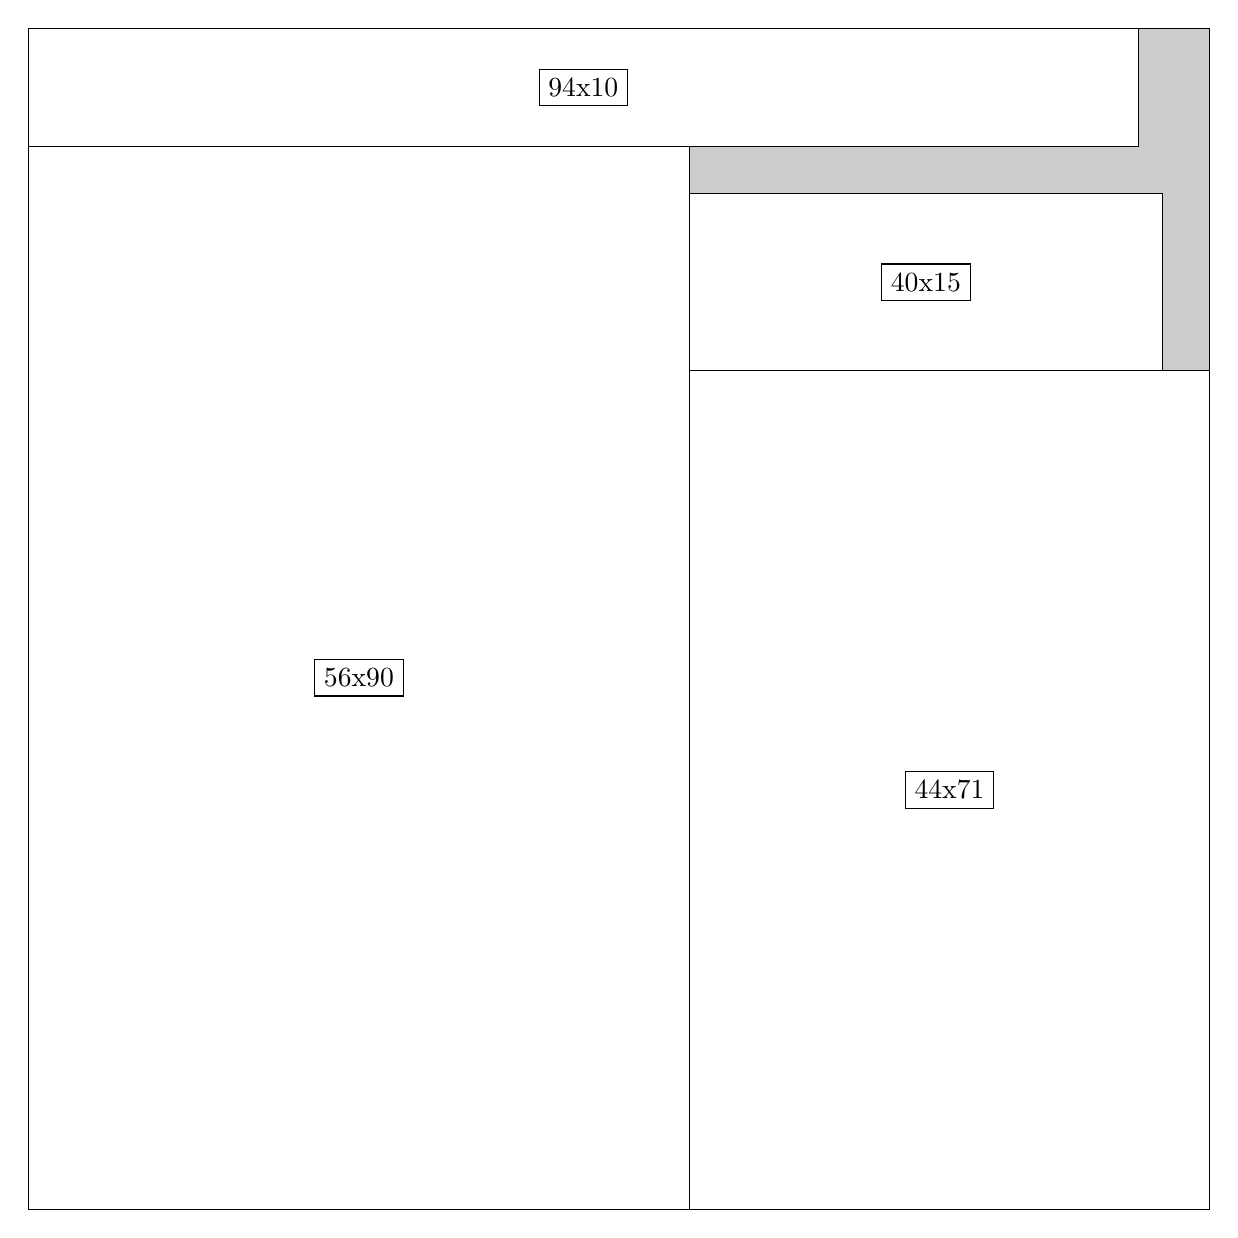
\begin{tikzpicture}[shorten >=1pt,scale=1.0,every node/.style={scale=1.0},->]
\tikzstyle{vertex}=[circle,fill=black!25,minimum size=14pt,inner sep=0pt]
\filldraw[fill=gray!40!white, draw=black] (0,0) rectangle (15.0,15.0);
\foreach \name/\x/\y/\w/\h in {56x90/0.0/0.0/8.4/13.5,44x71/8.4/0.0/6.6/10.65,94x10/0.0/13.5/14.1/1.5,40x15/8.4/10.65/6.0/2.25}
\filldraw[fill=white!40!white, draw=black] (\x,\y) rectangle node[draw] (\name) {\name} ++(\w,\h);
\end{tikzpicture}


w =56 , h =90 , x =0 , y =0 , v =5040
\par
w =44 , h =71 , x =56 , y =0 , v =3124
\par
w =94 , h =10 , x =0 , y =90 , v =940
\par
w =40 , h =15 , x =56 , y =71 , v =600
\par
\newpage


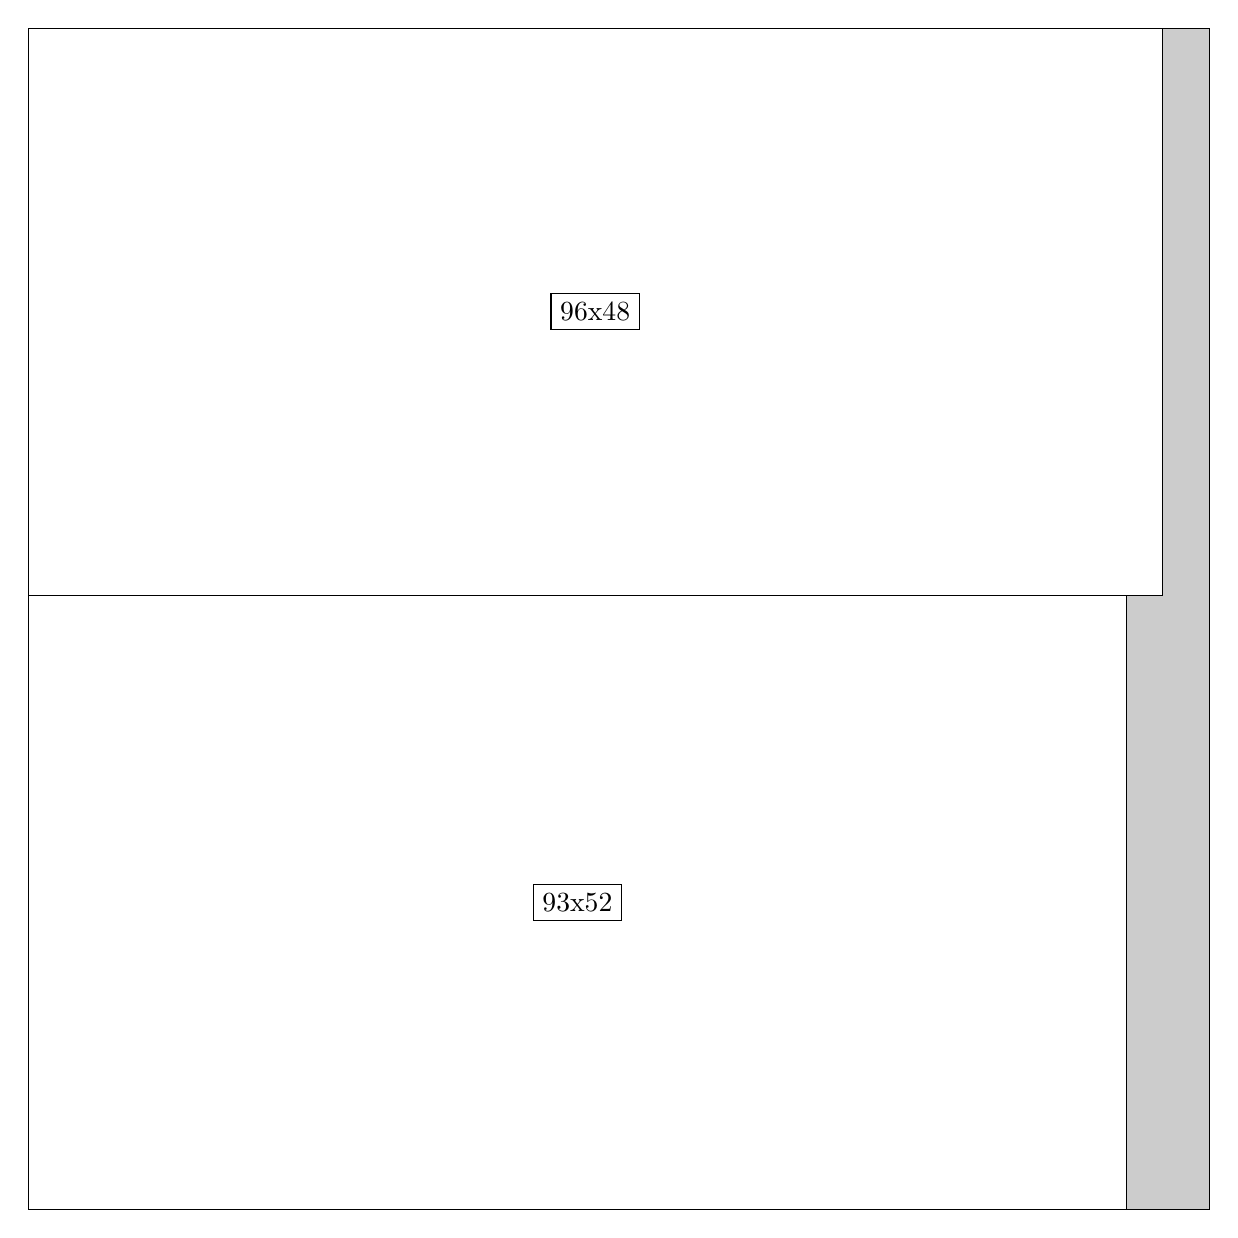
\begin{tikzpicture}[shorten >=1pt,scale=1.0,every node/.style={scale=1.0},->]
\tikzstyle{vertex}=[circle,fill=black!25,minimum size=14pt,inner sep=0pt]
\filldraw[fill=gray!40!white, draw=black] (0,0) rectangle (15.0,15.0);
\foreach \name/\x/\y/\w/\h in {93x52/0.0/0.0/13.95/7.8,96x48/0.0/7.8/14.399999999999999/7.199999999999999}
\filldraw[fill=white!40!white, draw=black] (\x,\y) rectangle node[draw] (\name) {\name} ++(\w,\h);
\end{tikzpicture}


w =93 , h =52 , x =0 , y =0 , v =4836
\par
w =96 , h =48 , x =0 , y =52 , v =4608
\par
\newpage


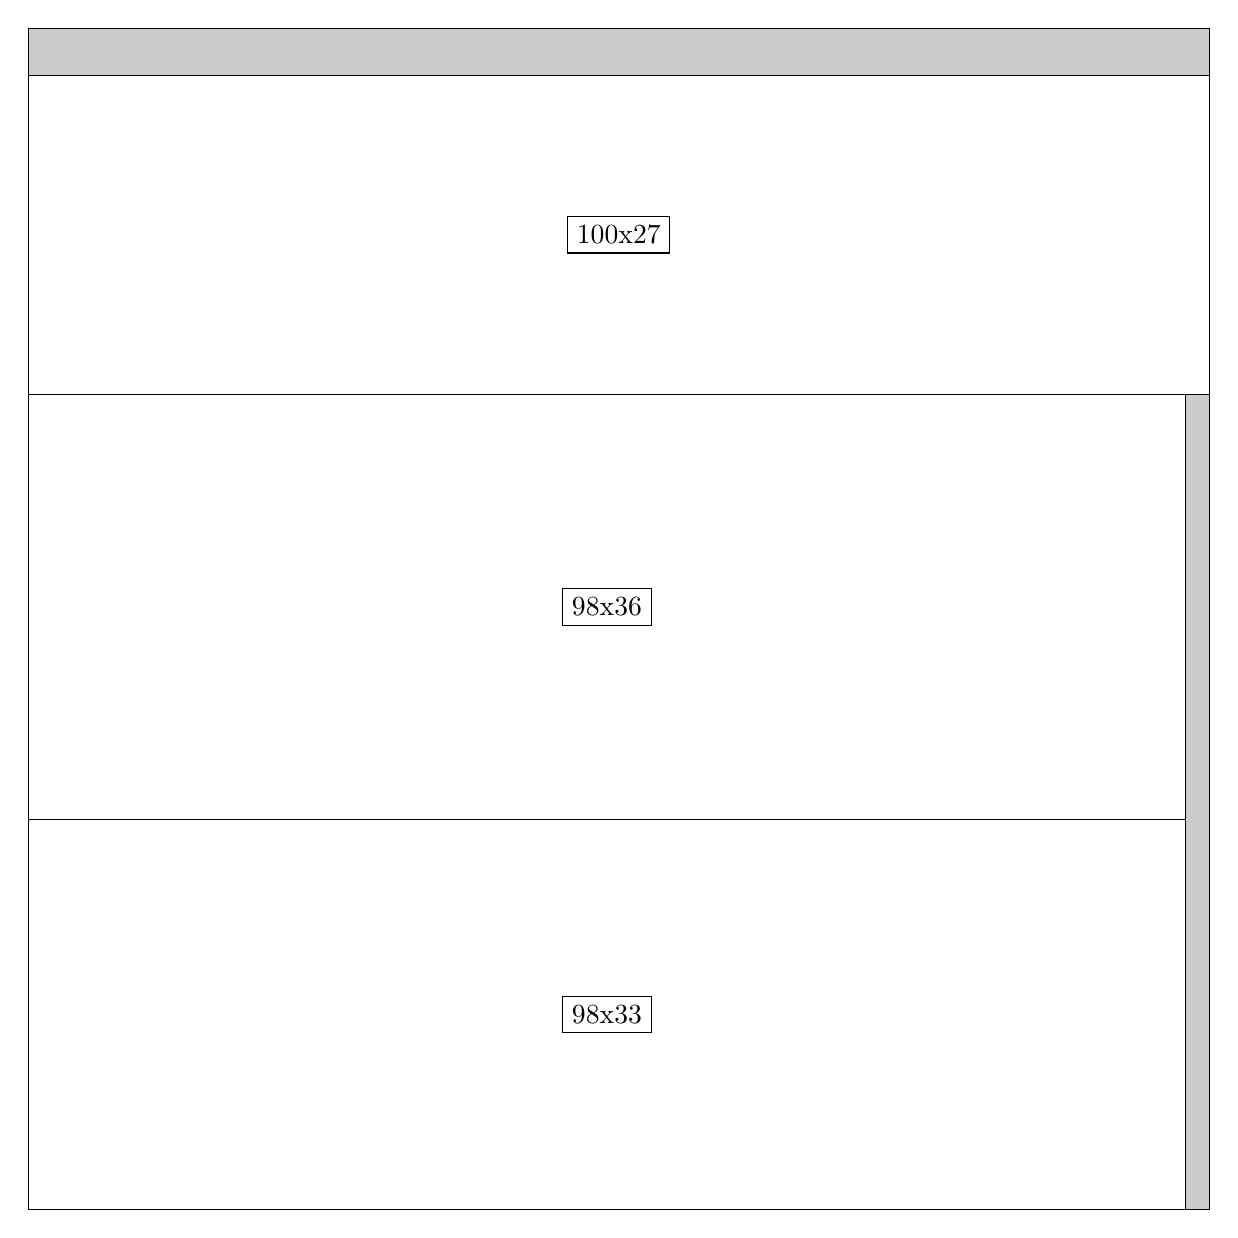
\begin{tikzpicture}[shorten >=1pt,scale=1.0,every node/.style={scale=1.0},->]
\tikzstyle{vertex}=[circle,fill=black!25,minimum size=14pt,inner sep=0pt]
\filldraw[fill=gray!40!white, draw=black] (0,0) rectangle (15.0,15.0);
\foreach \name/\x/\y/\w/\h in {98x36/0.0/4.95/14.7/5.3999999999999995,98x33/0.0/0.0/14.7/4.95,100x27/0.0/10.35/15.0/4.05}
\filldraw[fill=white!40!white, draw=black] (\x,\y) rectangle node[draw] (\name) {\name} ++(\w,\h);
\end{tikzpicture}


w =98 , h =36 , x =0 , y =33 , v =3528
\par
w =98 , h =33 , x =0 , y =0 , v =3234
\par
w =100 , h =27 , x =0 , y =69 , v =2700
\par
\newpage


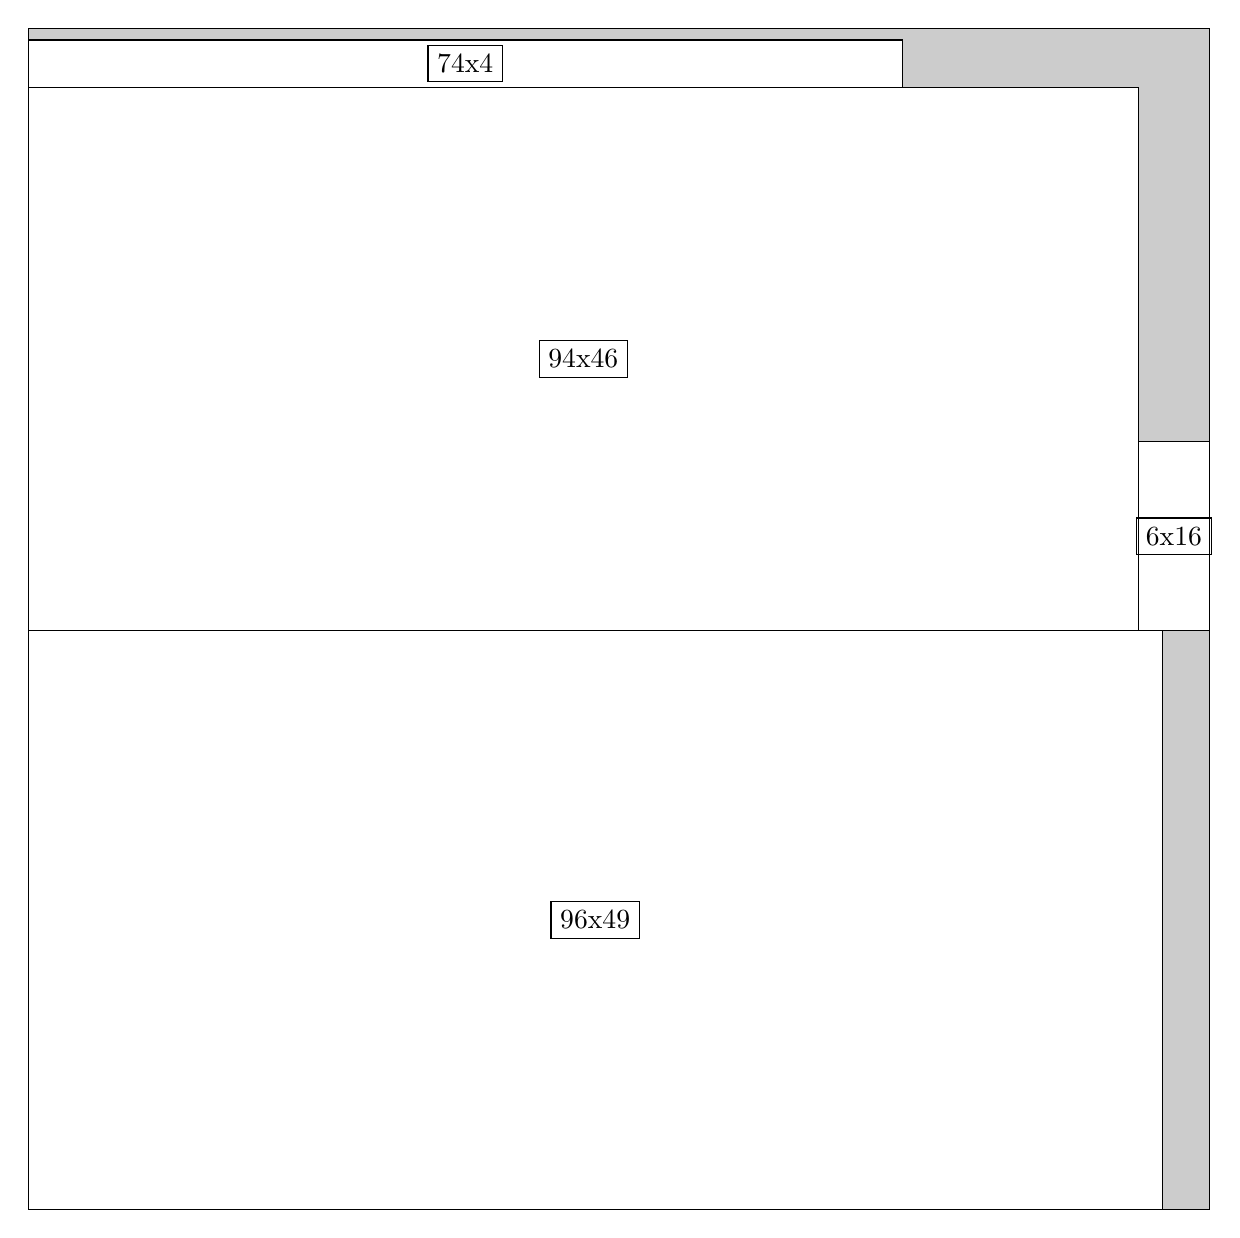
\begin{tikzpicture}[shorten >=1pt,scale=1.0,every node/.style={scale=1.0},->]
\tikzstyle{vertex}=[circle,fill=black!25,minimum size=14pt,inner sep=0pt]
\filldraw[fill=gray!40!white, draw=black] (0,0) rectangle (15.0,15.0);
\foreach \name/\x/\y/\w/\h in {96x49/0.0/0.0/14.399999999999999/7.35,94x46/0.0/7.35/14.1/6.8999999999999995,74x4/0.0/14.25/11.1/0.6,6x16/14.1/7.35/0.8999999999999999/2.4}
\filldraw[fill=white!40!white, draw=black] (\x,\y) rectangle node[draw] (\name) {\name} ++(\w,\h);
\end{tikzpicture}


w =96 , h =49 , x =0 , y =0 , v =4704
\par
w =94 , h =46 , x =0 , y =49 , v =4324
\par
w =74 , h =4 , x =0 , y =95 , v =296
\par
w =6 , h =16 , x =94 , y =49 , v =96
\par
\newpage


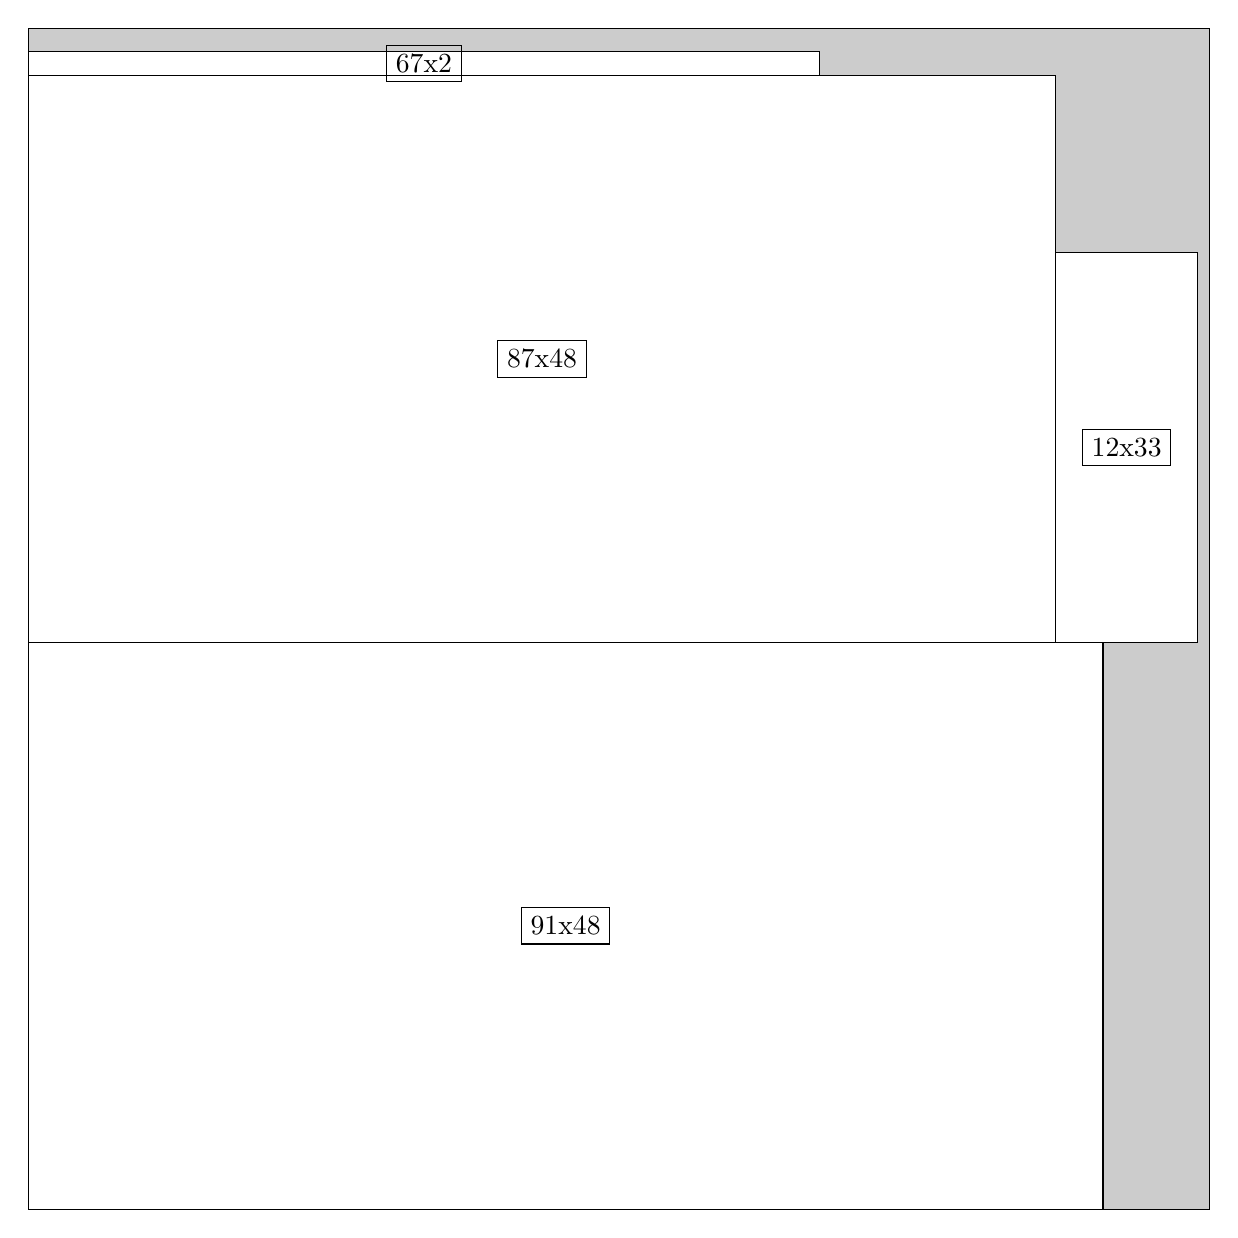
\begin{tikzpicture}[shorten >=1pt,scale=1.0,every node/.style={scale=1.0},->]
\tikzstyle{vertex}=[circle,fill=black!25,minimum size=14pt,inner sep=0pt]
\filldraw[fill=gray!40!white, draw=black] (0,0) rectangle (15.0,15.0);
\foreach \name/\x/\y/\w/\h in {91x48/0.0/0.0/13.65/7.199999999999999,87x48/0.0/7.199999999999999/13.049999999999999/7.199999999999999,12x33/13.049999999999999/7.199999999999999/1.7999999999999998/4.95,67x2/0.0/14.399999999999999/10.049999999999999/0.3}
\filldraw[fill=white!40!white, draw=black] (\x,\y) rectangle node[draw] (\name) {\name} ++(\w,\h);
\end{tikzpicture}


w =91 , h =48 , x =0 , y =0 , v =4368
\par
w =87 , h =48 , x =0 , y =48 , v =4176
\par
w =12 , h =33 , x =87 , y =48 , v =396
\par
w =67 , h =2 , x =0 , y =96 , v =134
\par
\newpage


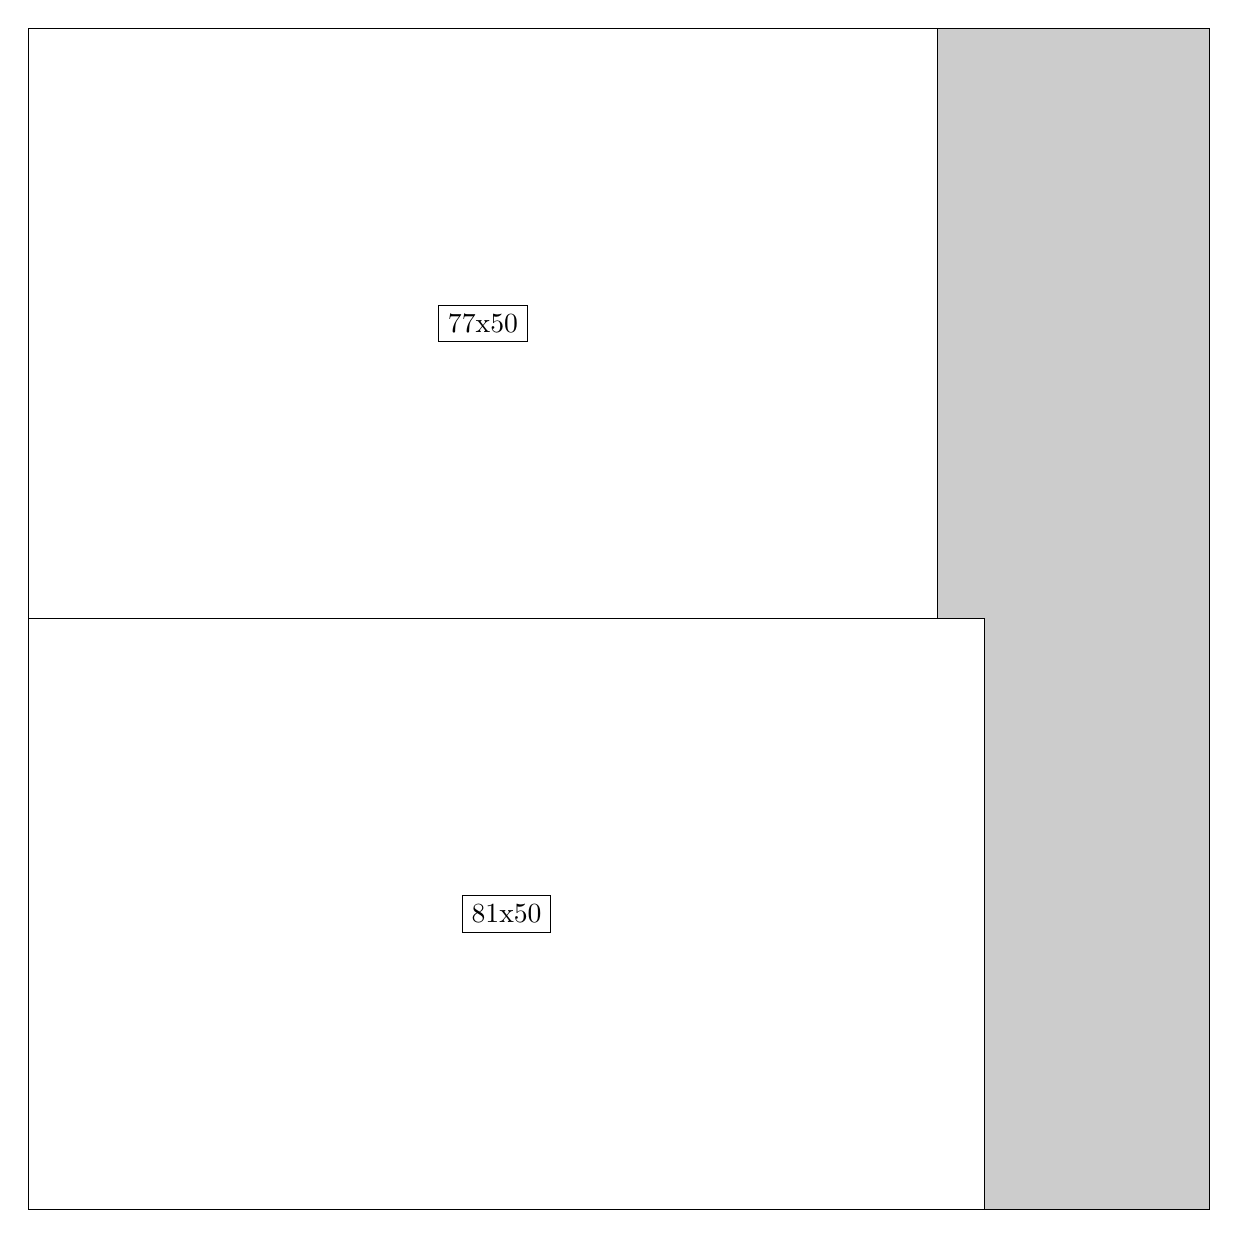
\begin{tikzpicture}[shorten >=1pt,scale=1.0,every node/.style={scale=1.0},->]
\tikzstyle{vertex}=[circle,fill=black!25,minimum size=14pt,inner sep=0pt]
\filldraw[fill=gray!40!white, draw=black] (0,0) rectangle (15.0,15.0);
\foreach \name/\x/\y/\w/\h in {81x50/0.0/0.0/12.15/7.5,77x50/0.0/7.5/11.549999999999999/7.5}
\filldraw[fill=white!40!white, draw=black] (\x,\y) rectangle node[draw] (\name) {\name} ++(\w,\h);
\end{tikzpicture}


w =81 , h =50 , x =0 , y =0 , v =4050
\par
w =77 , h =50 , x =0 , y =50 , v =3850
\par
\newpage


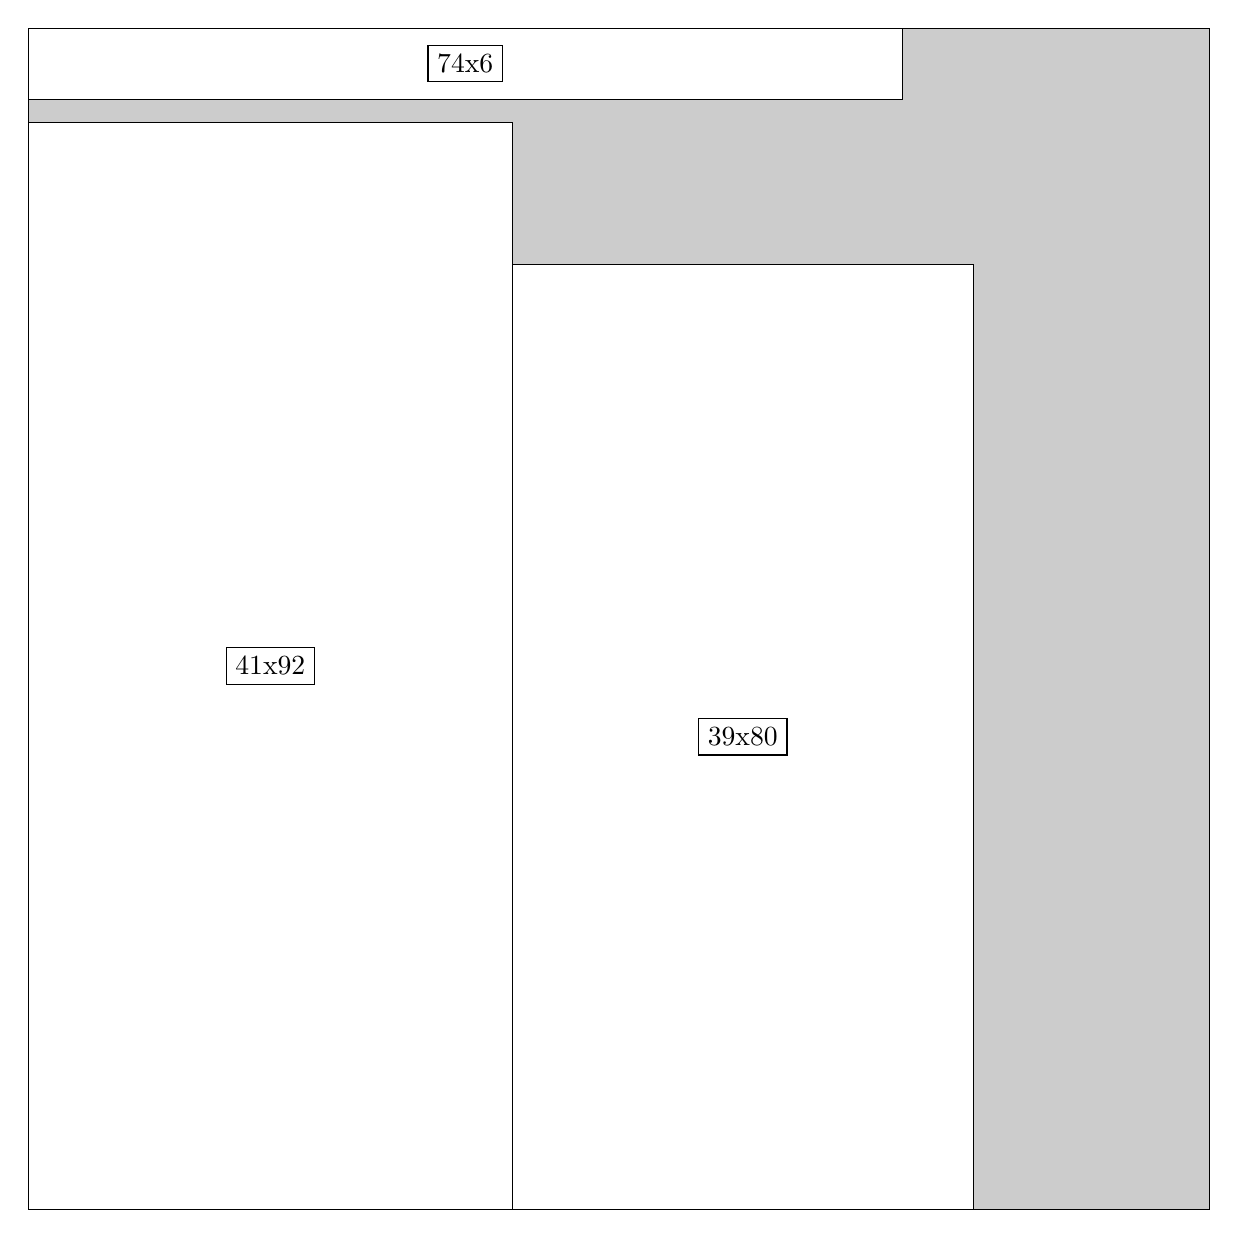
\begin{tikzpicture}[shorten >=1pt,scale=1.0,every node/.style={scale=1.0},->]
\tikzstyle{vertex}=[circle,fill=black!25,minimum size=14pt,inner sep=0pt]
\filldraw[fill=gray!40!white, draw=black] (0,0) rectangle (15.0,15.0);
\foreach \name/\x/\y/\w/\h in {41x92/0.0/0.0/6.1499999999999995/13.799999999999999,39x80/6.1499999999999995/0.0/5.85/12.0,74x6/0.0/14.1/11.1/0.8999999999999999}
\filldraw[fill=white!40!white, draw=black] (\x,\y) rectangle node[draw] (\name) {\name} ++(\w,\h);
\end{tikzpicture}


w =41 , h =92 , x =0 , y =0 , v =3772
\par
w =39 , h =80 , x =41 , y =0 , v =3120
\par
w =74 , h =6 , x =0 , y =94 , v =444
\par
\newpage


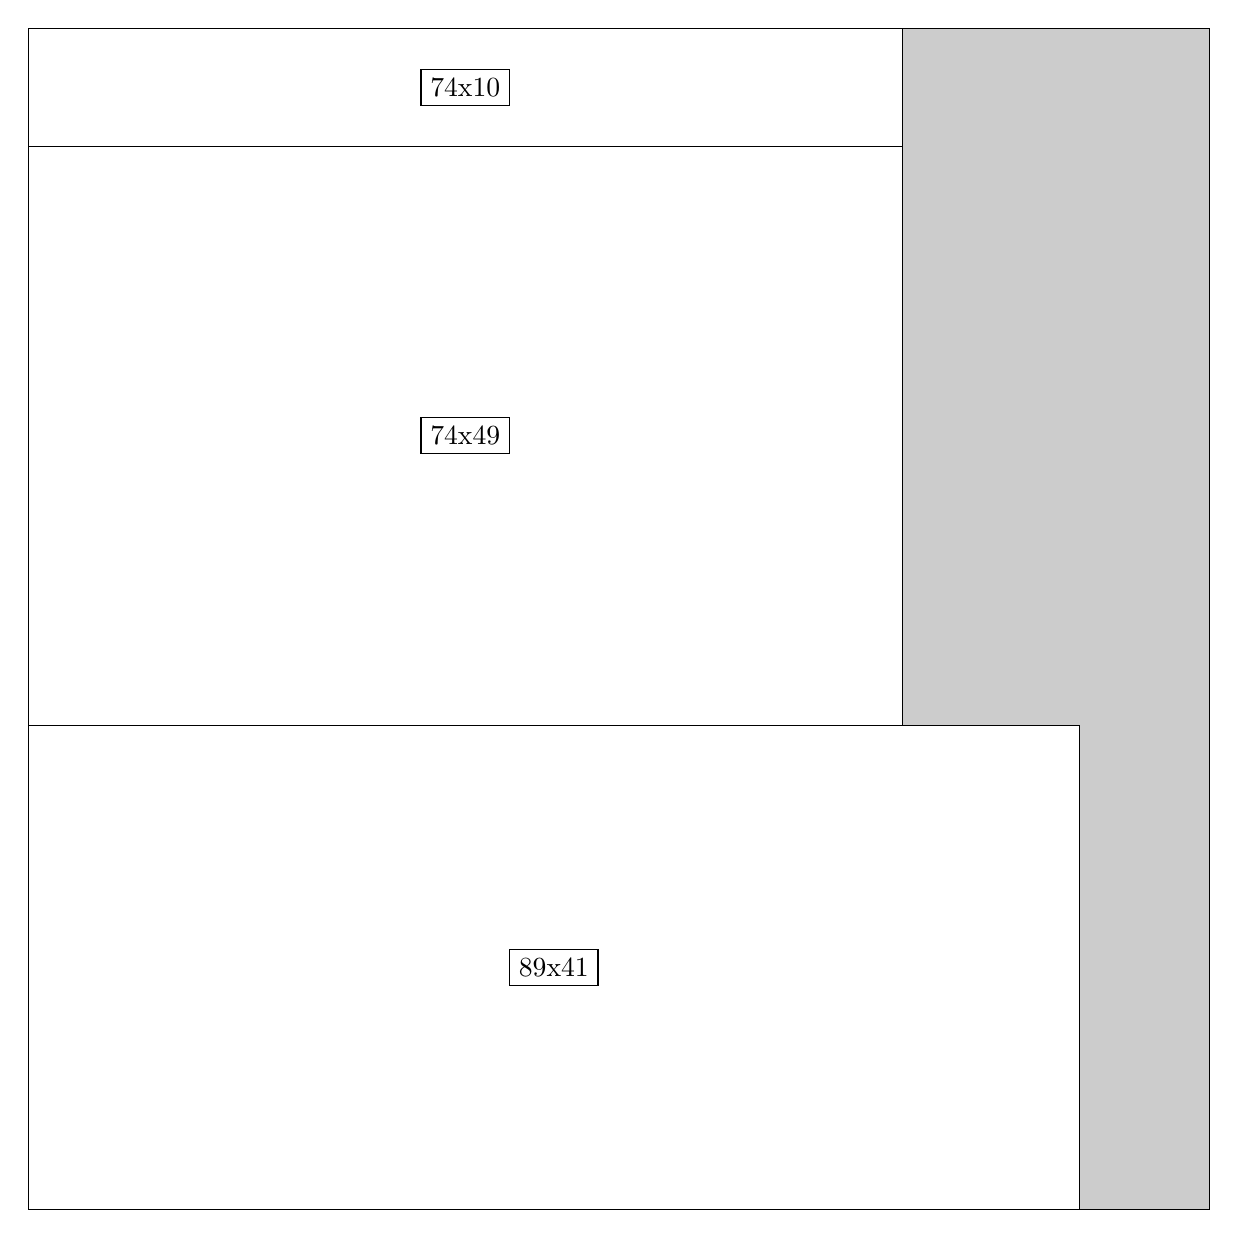
\begin{tikzpicture}[shorten >=1pt,scale=1.0,every node/.style={scale=1.0},->]
\tikzstyle{vertex}=[circle,fill=black!25,minimum size=14pt,inner sep=0pt]
\filldraw[fill=gray!40!white, draw=black] (0,0) rectangle (15.0,15.0);
\foreach \name/\x/\y/\w/\h in {74x10/0.0/13.5/11.1/1.5,89x41/0.0/0.0/13.35/6.1499999999999995,74x49/0.0/6.1499999999999995/11.1/7.35}
\filldraw[fill=white!40!white, draw=black] (\x,\y) rectangle node[draw] (\name) {\name} ++(\w,\h);
\end{tikzpicture}


w =74 , h =10 , x =0 , y =90 , v =740
\par
w =89 , h =41 , x =0 , y =0 , v =3649
\par
w =74 , h =49 , x =0 , y =41 , v =3626
\par
\newpage


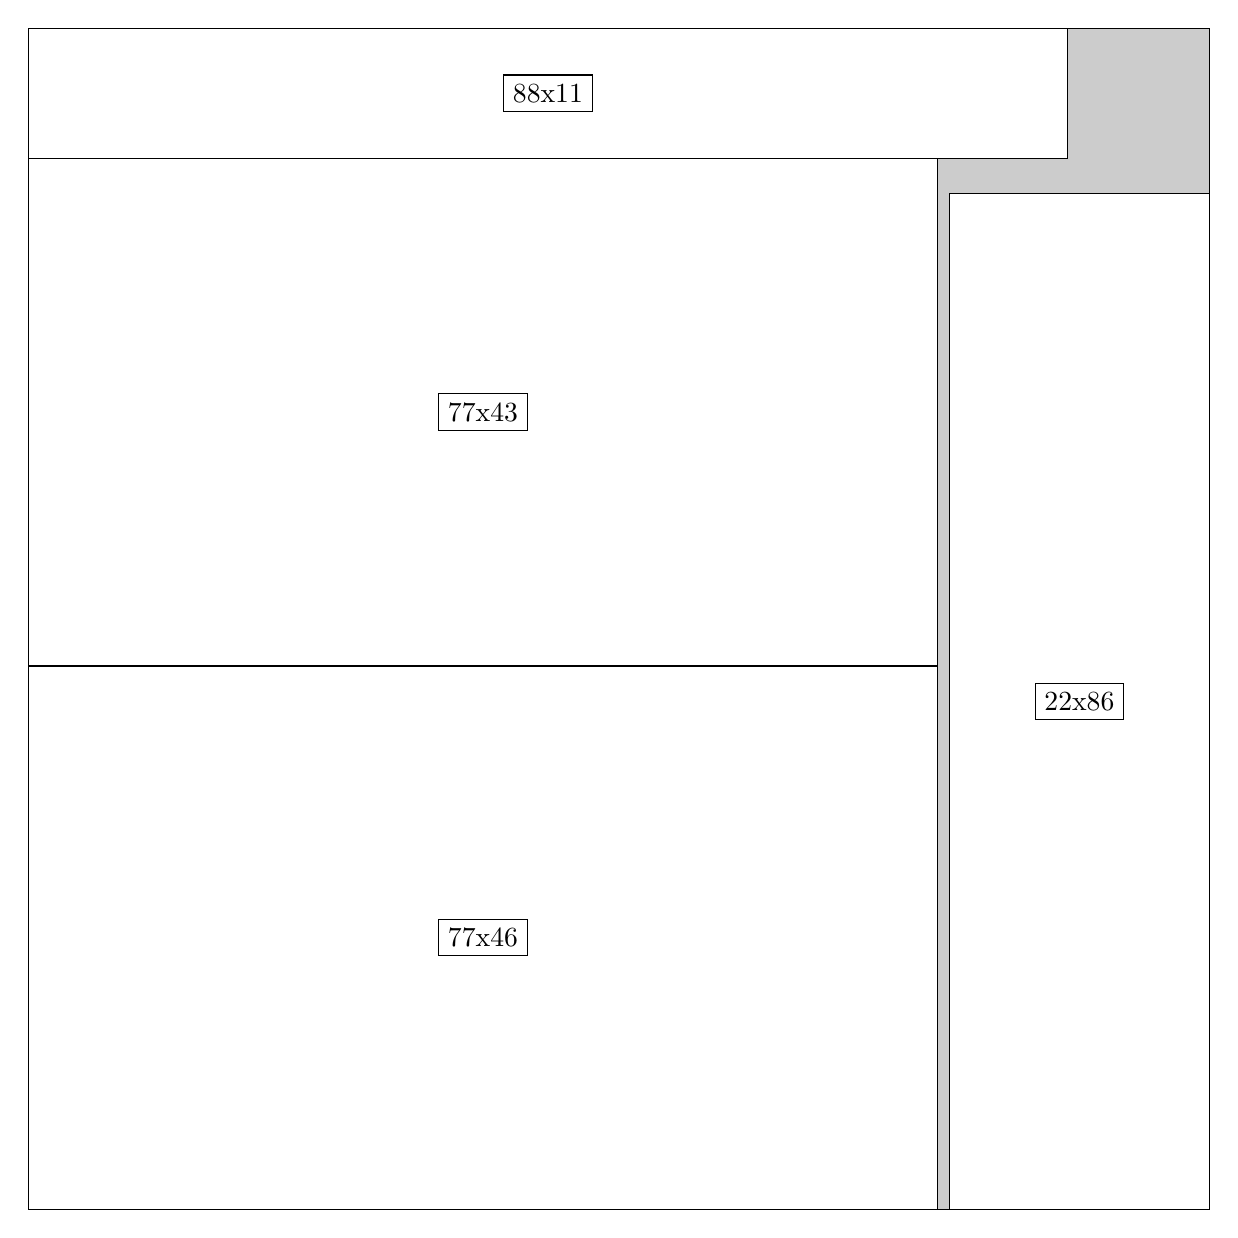
\begin{tikzpicture}[shorten >=1pt,scale=1.0,every node/.style={scale=1.0},->]
\tikzstyle{vertex}=[circle,fill=black!25,minimum size=14pt,inner sep=0pt]
\filldraw[fill=gray!40!white, draw=black] (0,0) rectangle (15.0,15.0);
\foreach \name/\x/\y/\w/\h in {77x46/0.0/0.0/11.549999999999999/6.8999999999999995,22x86/11.7/0.0/3.3/12.9,77x43/0.0/6.8999999999999995/11.549999999999999/6.45,88x11/0.0/13.35/13.2/1.65}
\filldraw[fill=white!40!white, draw=black] (\x,\y) rectangle node[draw] (\name) {\name} ++(\w,\h);
\end{tikzpicture}


w =77 , h =46 , x =0 , y =0 , v =3542
\par
w =22 , h =86 , x =78 , y =0 , v =1892
\par
w =77 , h =43 , x =0 , y =46 , v =3311
\par
w =88 , h =11 , x =0 , y =89 , v =968
\par
\newpage


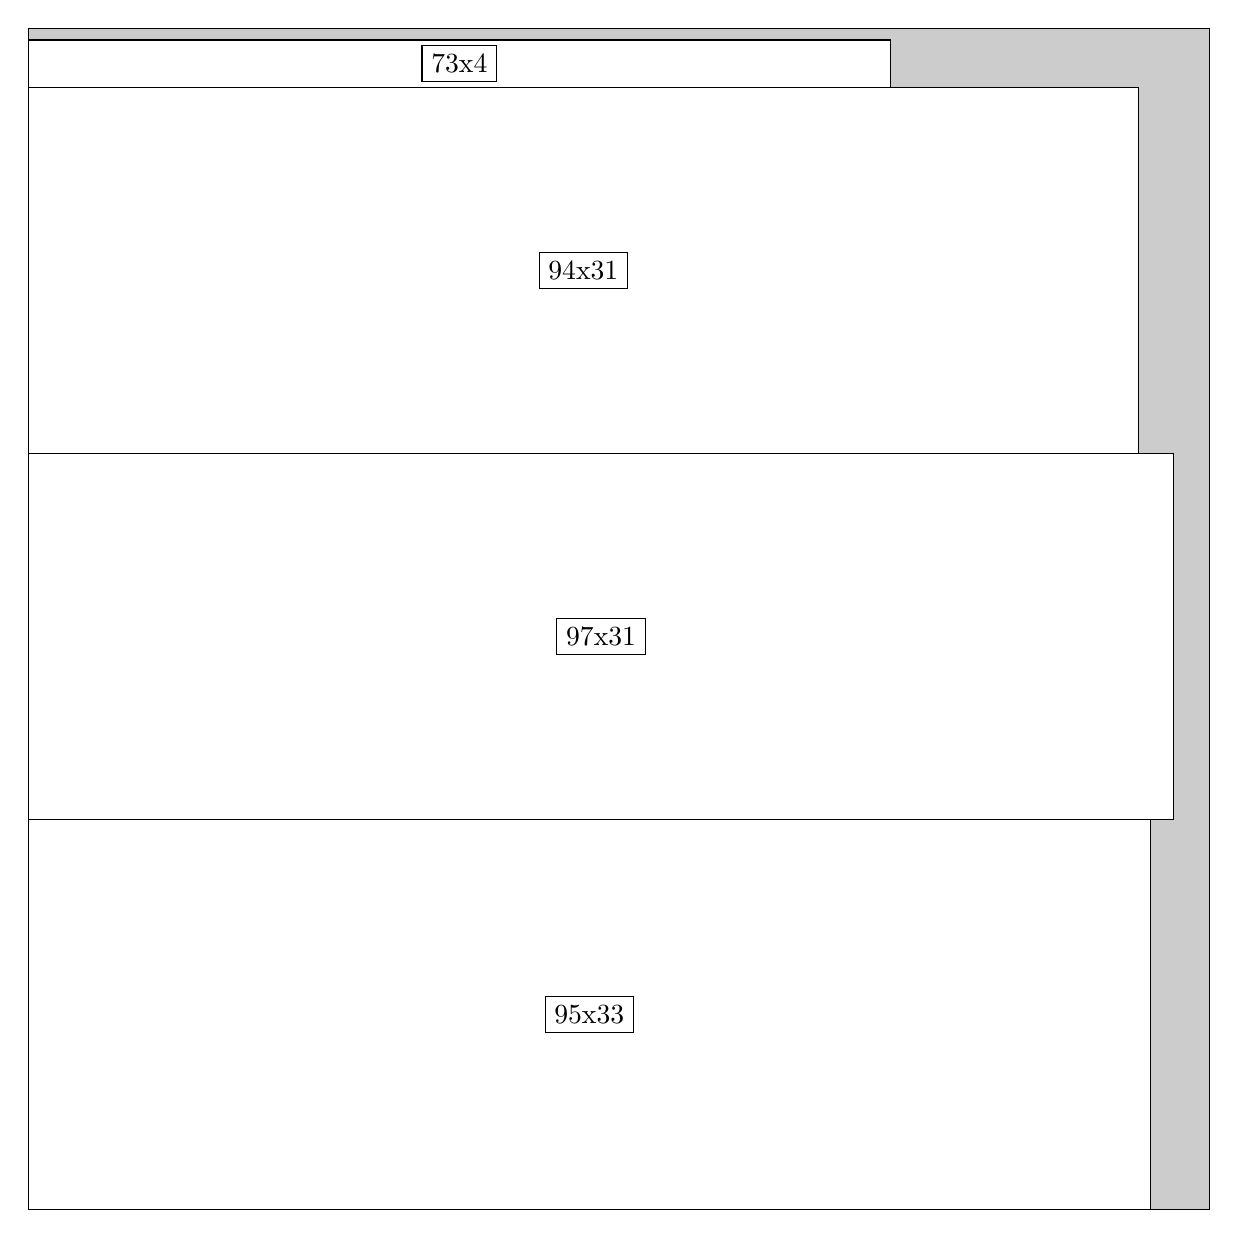
\begin{tikzpicture}[shorten >=1pt,scale=1.0,every node/.style={scale=1.0},->]
\tikzstyle{vertex}=[circle,fill=black!25,minimum size=14pt,inner sep=0pt]
\filldraw[fill=gray!40!white, draw=black] (0,0) rectangle (15.0,15.0);
\foreach \name/\x/\y/\w/\h in {95x33/0.0/0.0/14.25/4.95,97x31/0.0/4.95/14.549999999999999/4.6499999999999995,94x31/0.0/9.6/14.1/4.6499999999999995,73x4/0.0/14.25/10.95/0.6}
\filldraw[fill=white!40!white, draw=black] (\x,\y) rectangle node[draw] (\name) {\name} ++(\w,\h);
\end{tikzpicture}


w =95 , h =33 , x =0 , y =0 , v =3135
\par
w =97 , h =31 , x =0 , y =33 , v =3007
\par
w =94 , h =31 , x =0 , y =64 , v =2914
\par
w =73 , h =4 , x =0 , y =95 , v =292
\par
\newpage


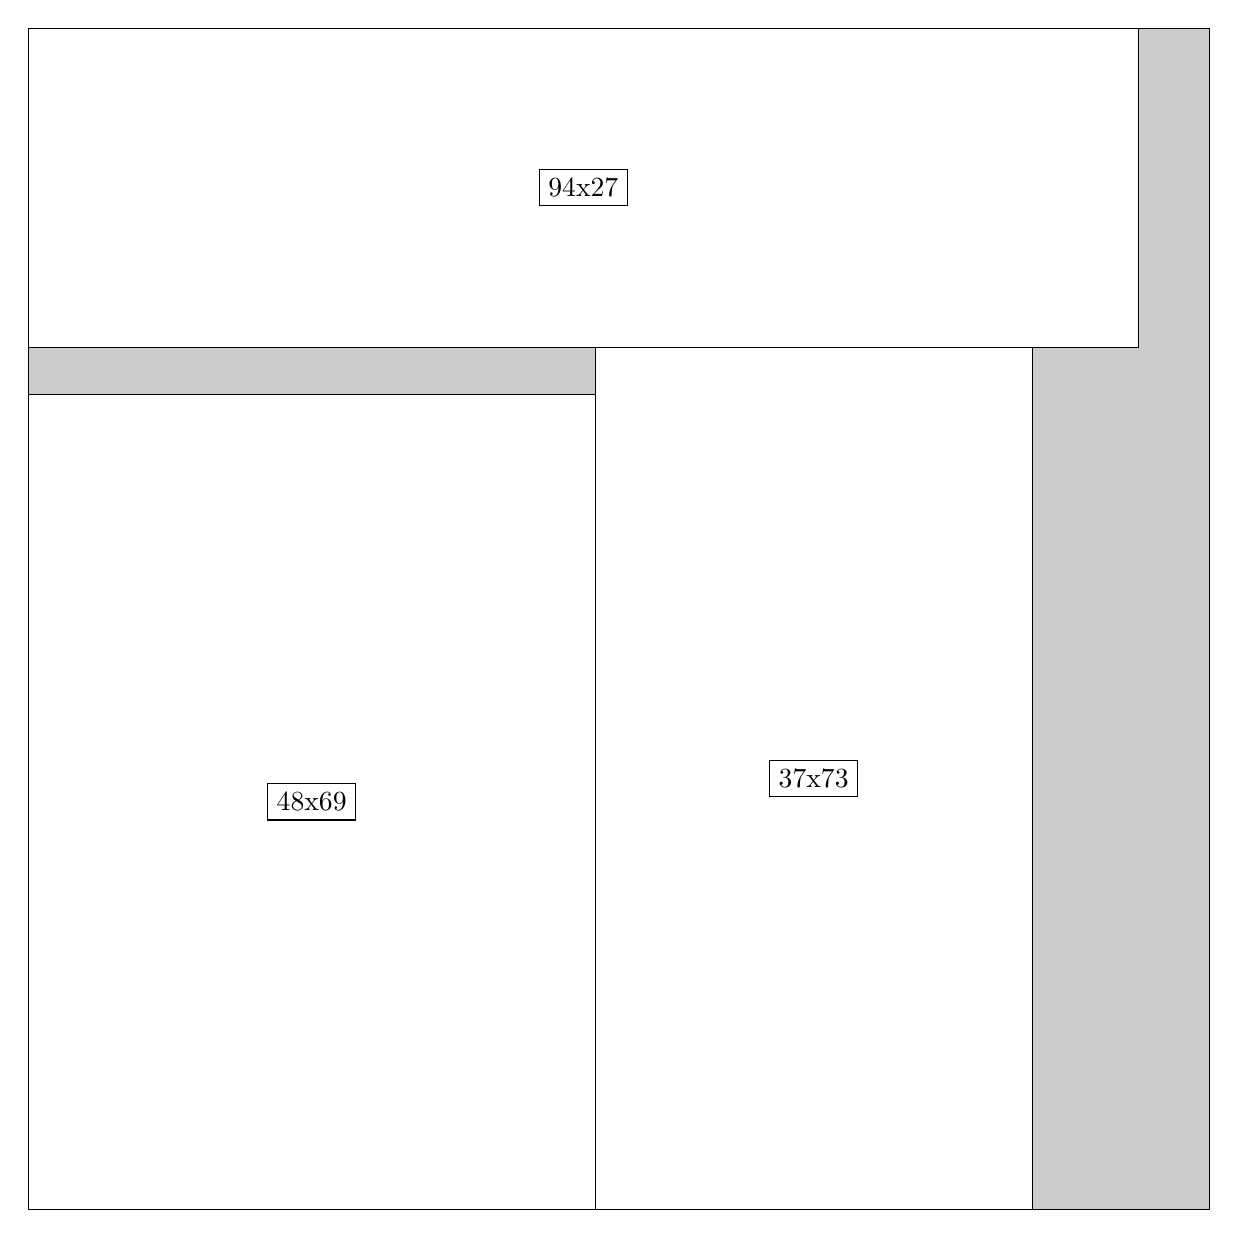
\begin{tikzpicture}[shorten >=1pt,scale=1.0,every node/.style={scale=1.0},->]
\tikzstyle{vertex}=[circle,fill=black!25,minimum size=14pt,inner sep=0pt]
\filldraw[fill=gray!40!white, draw=black] (0,0) rectangle (15.0,15.0);
\foreach \name/\x/\y/\w/\h in {48x69/0.0/0.0/7.199999999999999/10.35,37x73/7.199999999999999/0.0/5.55/10.95,94x27/0.0/10.95/14.1/4.05}
\filldraw[fill=white!40!white, draw=black] (\x,\y) rectangle node[draw] (\name) {\name} ++(\w,\h);
\end{tikzpicture}


w =48 , h =69 , x =0 , y =0 , v =3312
\par
w =37 , h =73 , x =48 , y =0 , v =2701
\par
w =94 , h =27 , x =0 , y =73 , v =2538
\par
\newpage


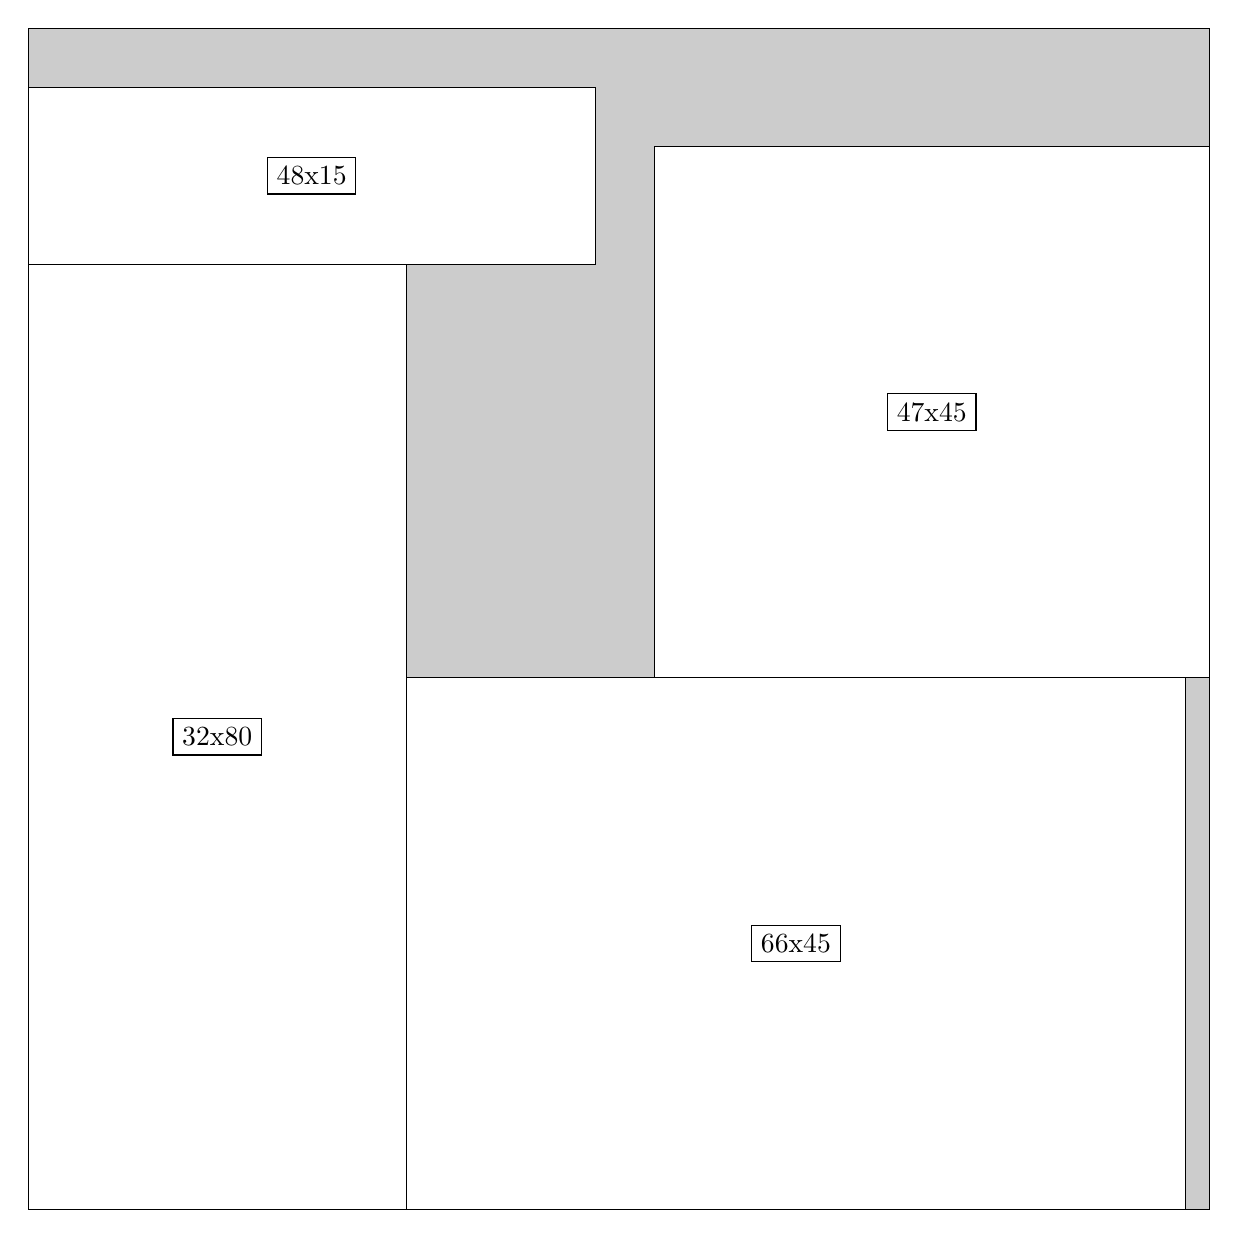
\begin{tikzpicture}[shorten >=1pt,scale=1.0,every node/.style={scale=1.0},->]
\tikzstyle{vertex}=[circle,fill=black!25,minimum size=14pt,inner sep=0pt]
\filldraw[fill=gray!40!white, draw=black] (0,0) rectangle (15.0,15.0);
\foreach \name/\x/\y/\w/\h in {32x80/0.0/0.0/4.8/12.0,66x45/4.8/0.0/9.9/6.75,47x45/7.949999999999999/6.75/7.05/6.75,48x15/0.0/12.0/7.199999999999999/2.25}
\filldraw[fill=white!40!white, draw=black] (\x,\y) rectangle node[draw] (\name) {\name} ++(\w,\h);
\end{tikzpicture}


w =32 , h =80 , x =0 , y =0 , v =2560
\par
w =66 , h =45 , x =32 , y =0 , v =2970
\par
w =47 , h =45 , x =53 , y =45 , v =2115
\par
w =48 , h =15 , x =0 , y =80 , v =720
\par
\newpage


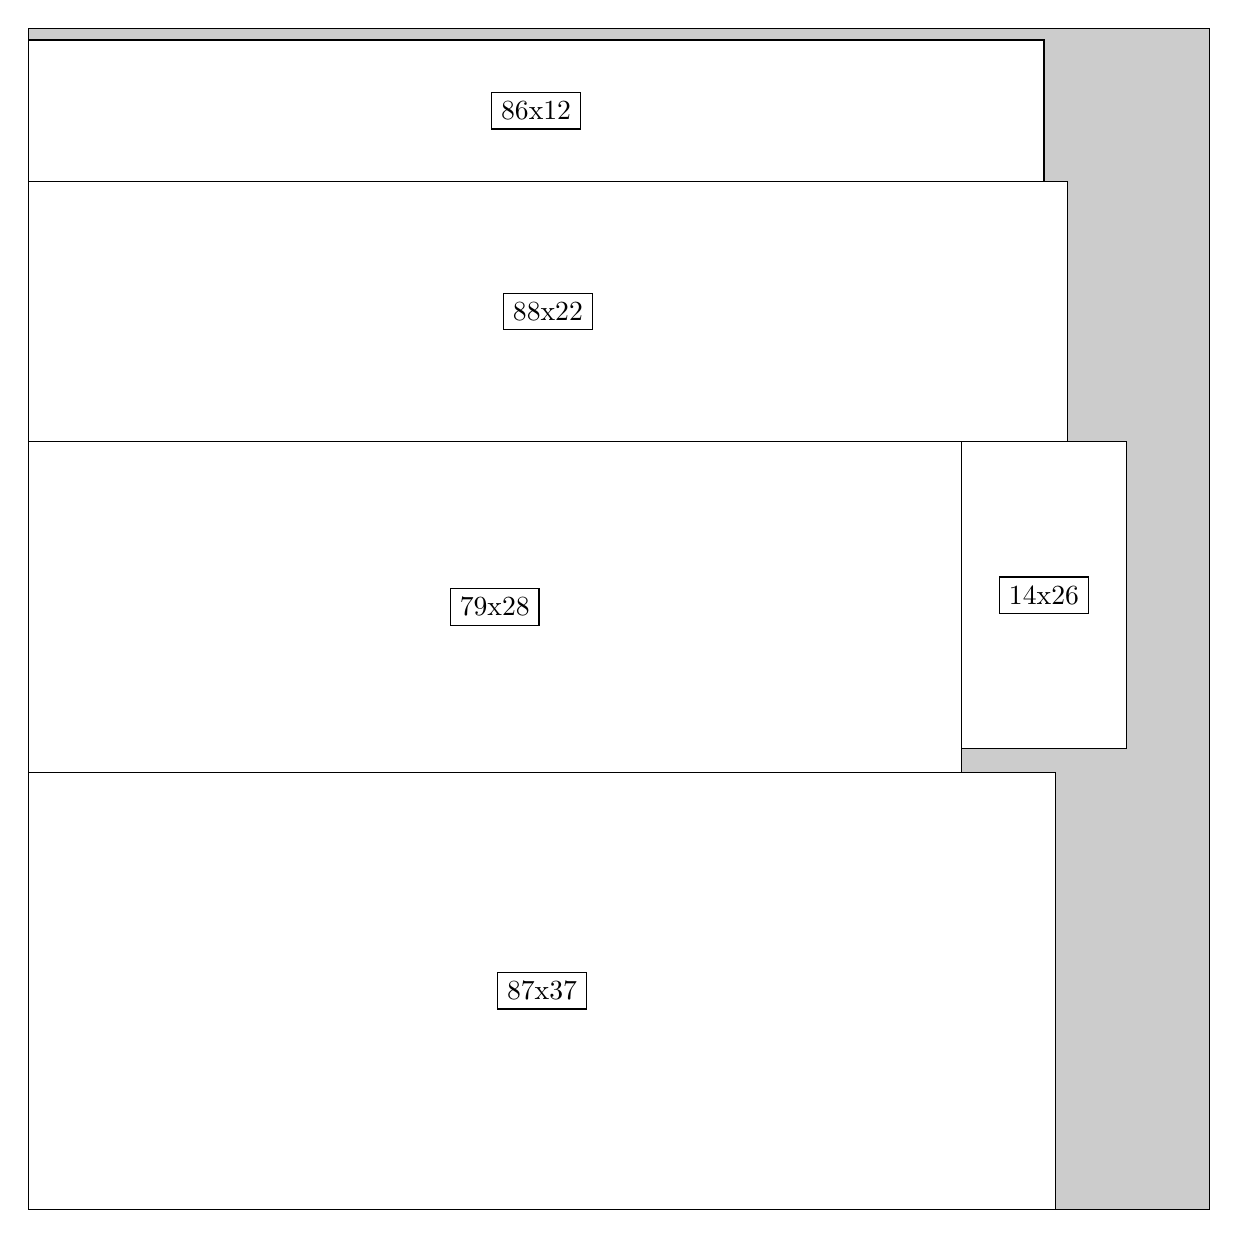
\begin{tikzpicture}[shorten >=1pt,scale=1.0,every node/.style={scale=1.0},->]
\tikzstyle{vertex}=[circle,fill=black!25,minimum size=14pt,inner sep=0pt]
\filldraw[fill=gray!40!white, draw=black] (0,0) rectangle (15.0,15.0);
\foreach \name/\x/\y/\w/\h in {87x37/0.0/0.0/13.049999999999999/5.55,79x28/0.0/5.55/11.85/4.2,88x22/0.0/9.75/13.2/3.3,86x12/0.0/13.049999999999999/12.9/1.7999999999999998,14x26/11.85/5.85/2.1/3.9}
\filldraw[fill=white!40!white, draw=black] (\x,\y) rectangle node[draw] (\name) {\name} ++(\w,\h);
\end{tikzpicture}


w =87 , h =37 , x =0 , y =0 , v =3219
\par
w =79 , h =28 , x =0 , y =37 , v =2212
\par
w =88 , h =22 , x =0 , y =65 , v =1936
\par
w =86 , h =12 , x =0 , y =87 , v =1032
\par
w =14 , h =26 , x =79 , y =39 , v =364
\par
\newpage


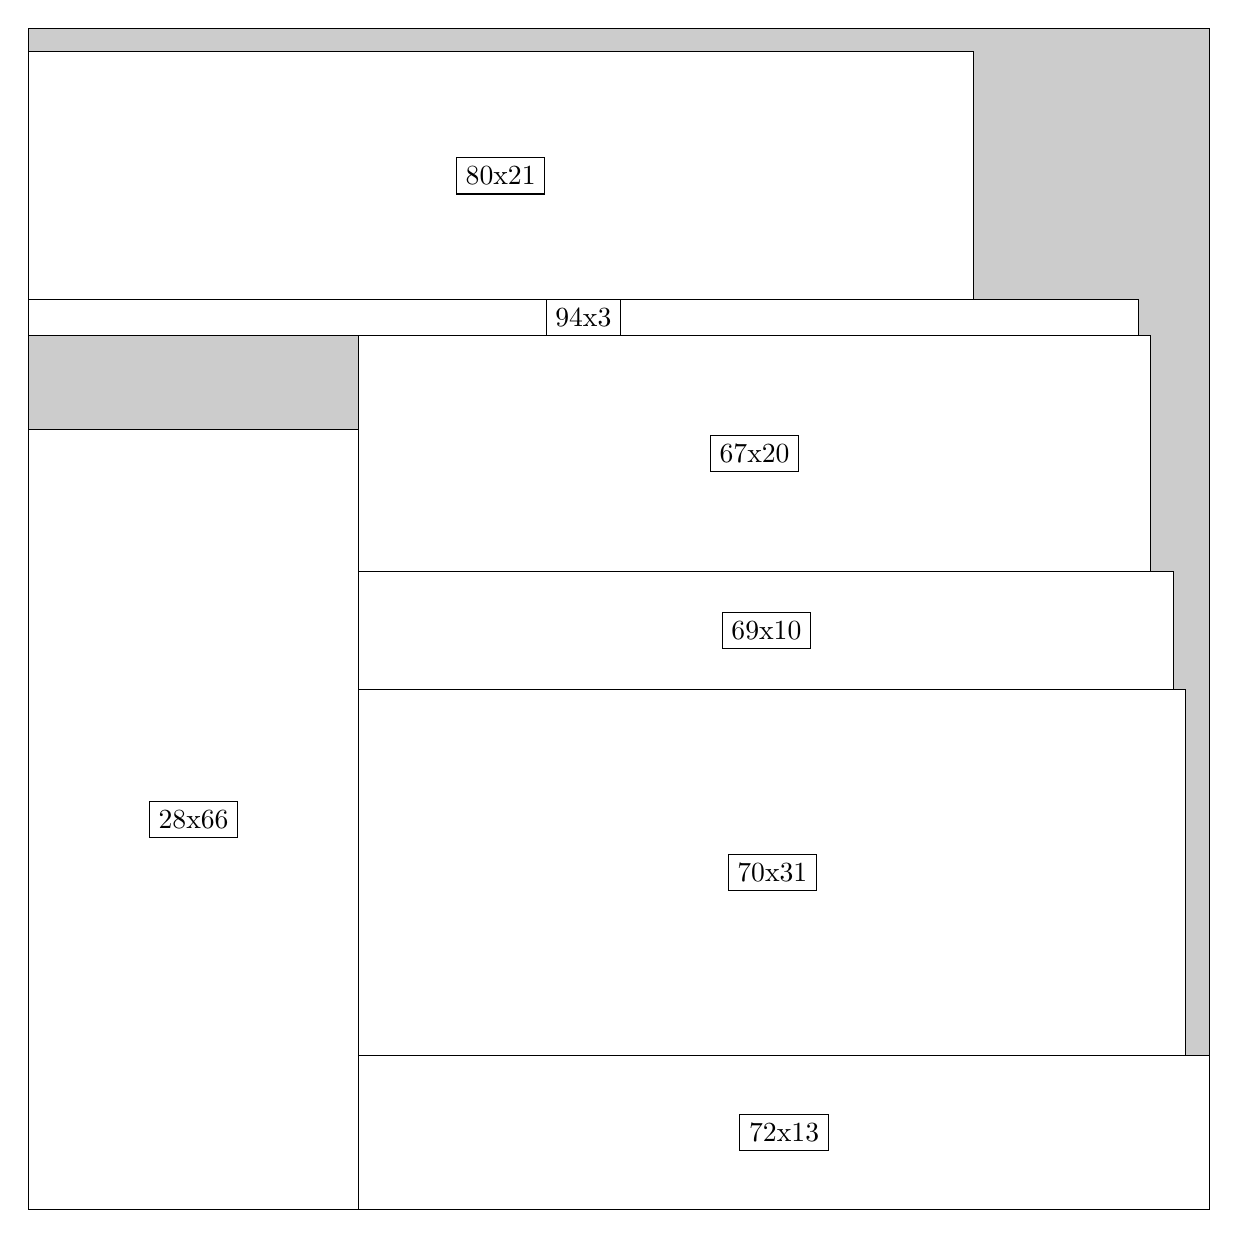
\begin{tikzpicture}[shorten >=1pt,scale=1.0,every node/.style={scale=1.0},->]
\tikzstyle{vertex}=[circle,fill=black!25,minimum size=14pt,inner sep=0pt]
\filldraw[fill=gray!40!white, draw=black] (0,0) rectangle (15.0,15.0);
\foreach \name/\x/\y/\w/\h in {28x66/0.0/0.0/4.2/9.9,70x31/4.2/1.95/10.5/4.6499999999999995,80x21/0.0/11.549999999999999/12.0/3.15,67x20/4.2/8.1/10.049999999999999/3.0,72x13/4.2/0.0/10.799999999999999/1.95,69x10/4.2/6.6/10.35/1.5,94x3/0.0/11.1/14.1/0.44999999999999996}
\filldraw[fill=white!40!white, draw=black] (\x,\y) rectangle node[draw] (\name) {\name} ++(\w,\h);
\end{tikzpicture}


w =28 , h =66 , x =0 , y =0 , v =1848
\par
w =70 , h =31 , x =28 , y =13 , v =2170
\par
w =80 , h =21 , x =0 , y =77 , v =1680
\par
w =67 , h =20 , x =28 , y =54 , v =1340
\par
w =72 , h =13 , x =28 , y =0 , v =936
\par
w =69 , h =10 , x =28 , y =44 , v =690
\par
w =94 , h =3 , x =0 , y =74 , v =282
\par
\newpage


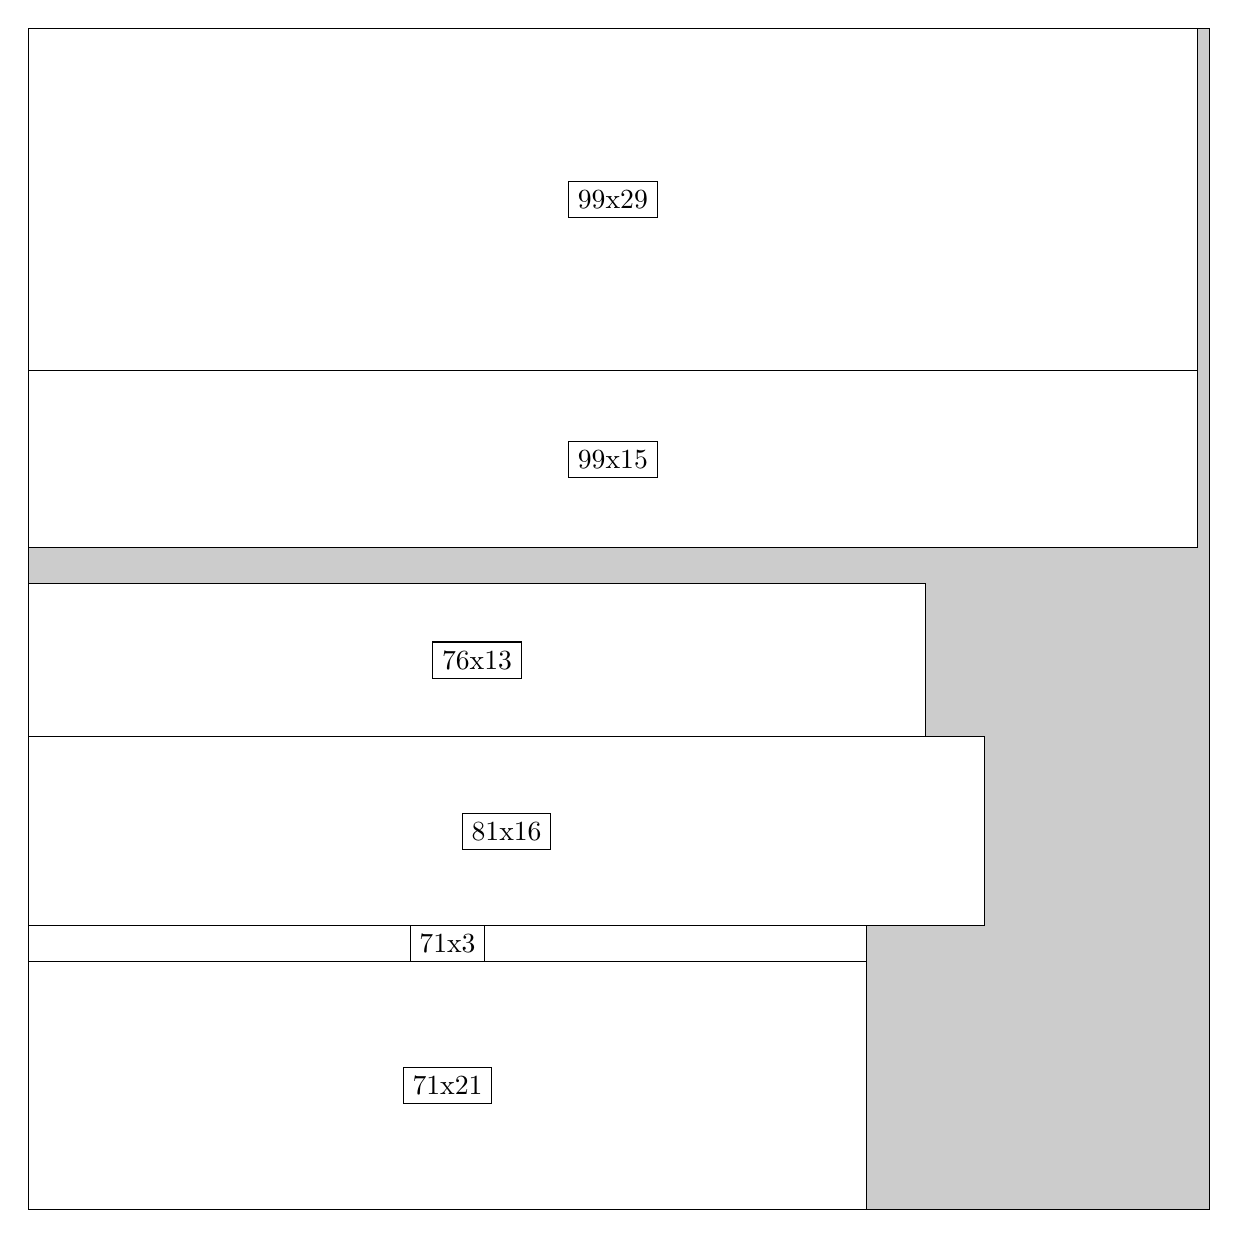
\begin{tikzpicture}[shorten >=1pt,scale=1.0,every node/.style={scale=1.0},->]
\tikzstyle{vertex}=[circle,fill=black!25,minimum size=14pt,inner sep=0pt]
\filldraw[fill=gray!40!white, draw=black] (0,0) rectangle (15.0,15.0);
\foreach \name/\x/\y/\w/\h in {99x29/0.0/10.65/14.85/4.35,71x21/0.0/0.0/10.65/3.15,99x15/0.0/8.4/14.85/2.25,81x16/0.0/3.5999999999999996/12.15/2.4,76x13/0.0/6.0/11.4/1.95,71x3/0.0/3.15/10.65/0.44999999999999996}
\filldraw[fill=white!40!white, draw=black] (\x,\y) rectangle node[draw] (\name) {\name} ++(\w,\h);
\end{tikzpicture}


w =99 , h =29 , x =0 , y =71 , v =2871
\par
w =71 , h =21 , x =0 , y =0 , v =1491
\par
w =99 , h =15 , x =0 , y =56 , v =1485
\par
w =81 , h =16 , x =0 , y =24 , v =1296
\par
w =76 , h =13 , x =0 , y =40 , v =988
\par
w =71 , h =3 , x =0 , y =21 , v =213
\par
\newpage


\end{document}